
%% bare_conf.tex
%% V1.4b
%% 2015/08/26
%% by Michael Shell
%% See:
%% http://www.michaelshell.org/
%% for current contact information.
%%
%% This is a skeleton file demonstrating the use of IEEEtran.cls
%% (requires IEEEtran.cls version 1.8b or later) with an IEEE
%% conference paper.
%%
%% Support sites:
%% http://www.michaelshell.org/tex/ieeetran/
%% http://www.ctan.org/pkg/ieeetran
%% and
%% http://www.ieee.org/

%%*************************************************************************
%% Legal Notice:
%% This code is offered as-is without any warranty either expressed or
%% implied; without even the implied warranty of MERCHANTABILITY or
%% FITNESS FOR A PARTICULAR PURPOSE! 
%% User assumes all risk.
%% In no event shall the IEEE or any contributor to this code be liable for
%% any damages or losses, including, but not limited to, incidental,
%% consequential, or any other damages, resulting from the use or misuse
%% of any information contained here.
%%
%% All comments are the opinions of their respective authors and are not
%% necessarily endorsed by the IEEE.
%%
%% This work is distributed under the LaTeX Project Public License (LPPL)
%% ( http://www.latex-project.org/ ) version 1.3, and may be freely used,
%% distributed and modified. A copy of the LPPL, version 1.3, is included
%% in the base LaTeX documentation of all distributions of LaTeX released
%% 2003/12/01 or later.
%% Retain all contribution notices and credits.
%% ** Modified files should be clearly indicated as such, including  **
%% ** renaming them and changing author support contact information. **
%%*************************************************************************


% *** Authors should verify (and, if needed, correct) their LaTeX system  ***
% *** with the testflow diagnostic prior to trusting their LaTeX platform ***
% *** with production work. The IEEE's font choices and paper sizes can   ***
% *** trigger bugs that do not appear when using other class files.       ***                          ***
% The testflow support page is at:
% http://www.michaelshell.org/tex/testflow/



\documentclass[conference]{IEEEtran}
% Some Computer Society conferences also require the compsoc mode option,
% but others use the standard conference format.
%
% If IEEEtran.cls has not been installed into the LaTeX system files,
% manually specify the path to it like:
% \documentclass[conference]{../sty/IEEEtran}





% Some very useful LaTeX packages include:
% (uncomment the ones you want to load)


% *** MISC UTILITY PACKAGES ***
%
%\usepackage{ifpdf}
% Heiko Oberdiek's ifpdf.sty is very useful if you need conditional
% compilation based on whether the output is pdf or dvi.
% usage:
% \ifpdf
%   % pdf code
% \else
%   % dvi code
% \fi
% The latest version of ifpdf.sty can be obtained from:
% http://www.ctan.org/pkg/ifpdf
% Also, note that IEEEtran.cls V1.7 and later provides a builtin
% \ifCLASSINFOpdf conditional that works the same way.
% When switching from latex to pdflatex and vice-versa, the compiler may
% have to be run twice to clear warning/error messages.






% *** CITATION PACKAGES ***
%
%\usepackage{cite}
% cite.sty was written by Donald Arseneau
% V1.6 and later of IEEEtran pre-defines the format of the cite.sty package
% \cite{} output to follow that of the IEEE. Loading the cite package will
% result in citation numbers being automatically sorted and properly
% "compressed/ranged". e.g., [1], [9], [2], [7], [5], [6] without using
% cite.sty will become [1], [2], [5]--[7], [9] using cite.sty. cite.sty's
% \cite will automatically add leading space, if needed. Use cite.sty's
% noadjust option (cite.sty V3.8 and later) if you want to turn this off
% such as if a citation ever needs to be enclosed in parenthesis.
% cite.sty is already installed on most LaTeX systems. Be sure and use
% version 5.0 (2009-03-20) and later if using hyperref.sty.
% The latest version can be obtained at:
% http://www.ctan.org/pkg/cite
% The documentation is contained in the cite.sty file itself.






% *** GRAPHICS RELATED PACKAGES ***
%
\ifCLASSINFOpdf
  % \usepackage[pdftex]{graphicx}
  % declare the path(s) where your graphic files are
  % \graphicspath{{../pdf/}{../jpeg/}}
  % and their extensions so you won't have to specify these with
  % every instance of \includegraphics
  % \DeclareGraphicsExtensions{.pdf,.jpeg,.png}
\else
  % or other class option (dvipsone, dvipdf, if not using dvips). graphicx
  % will default to the driver specified in the system graphics.cfg if no
  % driver is specified.
  % \usepackage[dvips]{graphicx}
  % declare the path(s) where your graphic files are
  % \graphicspath{{../eps/}}
  % and their extensions so you won't have to specify these with
  % every instance of \includegraphics
  % \DeclareGraphicsExtensions{.eps}
\fi
% graphicx was written by David Carlisle and Sebastian Rahtz. It is
% required if you want graphics, photos, etc. graphicx.sty is already
% installed on most LaTeX systems. The latest version and documentation
% can be obtained at: 
% http://www.ctan.org/pkg/graphicx
% Another good source of documentation is "Using Imported Graphics in
% LaTeX2e" by Keith Reckdahl which can be found at:
% http://www.ctan.org/pkg/epslatex
%
% latex, and pdflatex in dvi mode, support graphics in encapsulated
% postscript (.eps) format. pdflatex in pdf mode supports graphics
% in .pdf, .jpeg, .png and .mps (metapost) formats. Users should ensure
% that all non-photo figures use a vector format (.eps, .pdf, .mps) and
% not a bitmapped formats (.jpeg, .png). The IEEE frowns on bitmapped formats
% which can result in "jaggedy"/blurry rendering of lines and letters as
% well as large increases in file sizes.
%
% You can find documentation about the pdfTeX application at:
% http://www.tug.org/applications/pdftex





% *** MATH PACKAGES ***
%
%\usepackage{amsmath}
% A popular package from the American Mathematical Society that provides
% many useful and powerful commands for dealing with mathematics.
%
% Note that the amsmath package sets \interdisplaylinepenalty to 10000
% thus preventing page breaks from occurring within multiline equations. Use:
%\interdisplaylinepenalty=2500
% after loading amsmath to restore such page breaks as IEEEtran.cls normally
% does. amsmath.sty is already installed on most LaTeX systems. The latest
% version and documentation can be obtained at:
% http://www.ctan.org/pkg/amsmath





% *** SPECIALIZED LIST PACKAGES ***
%
%\usepackage{algorithmic}
% algorithmic.sty was written by Peter Williams and Rogerio Brito.
% This package provides an algorithmic environment fo describing algorithms.
% You can use the algorithmic environment in-text or within a figure
% environment to provide for a floating algorithm. Do NOT use the algorithm
% floating environment provided by algorithm.sty (by the same authors) or
% algorithm2e.sty (by Christophe Fiorio) as the IEEE does not use dedicated
% algorithm float types and packages that provide these will not provide
% correct IEEE style captions. The latest version and documentation of
% algorithmic.sty can be obtained at:
% http://www.ctan.org/pkg/algorithms
% Also of interest may be the (relatively newer and more customizable)
% algorithmicx.sty package by Szasz Janos:
% http://www.ctan.org/pkg/algorithmicx




% *** ALIGNMENT PACKAGES ***
%
%\usepackage{array}
% Frank Mittelbach's and David Carlisle's array.sty patches and improves
% the standard LaTeX2e array and tabular environments to provide better
% appearance and additional user controls. As the default LaTeX2e table
% generation code is lacking to the point of almost being broken with
% respect to the quality of the end results, all users are strongly
% advised to use an enhanced (at the very least that provided by array.sty)
% set of table tools. array.sty is already installed on most systems. The
% latest version and documentation can be obtained at:
% http://www.ctan.org/pkg/array


% IEEEtran contains the IEEEeqnarray family of commands that can be used to
% generate multiline equations as well as matrices, tables, etc., of high
% quality.




% *** SUBFIGURE PACKAGES ***
%\ifCLASSOPTIONcompsoc
%  \usepackage[caption=false,font=normalsize,labelfont=sf,textfont=sf]{subfig}
%\else
%  \usepackage[caption=false,font=footnotesize]{subfig}
%\fi
% subfig.sty, written by Steven Douglas Cochran, is the modern replacement
% for subfigure.sty, the latter of which is no longer maintained and is
% incompatible with some LaTeX packages including fixltx2e. However,
% subfig.sty requires and automatically loads Axel Sommerfeldt's caption.sty
% which will override IEEEtran.cls' handling of captions and this will result
% in non-IEEE style figure/table captions. To prevent this problem, be sure
% and invoke subfig.sty's "caption=false" package option (available since
% subfig.sty version 1.3, 2005/06/28) as this is will preserve IEEEtran.cls
% handling of captions.
% Note that the Computer Society format requires a larger sans serif font
% than the serif footnote size font used in traditional IEEE formatting
% and thus the need to invoke different subfig.sty package options depending
% on whether compsoc mode has been enabled.
%
% The latest version and documentation of subfig.sty can be obtained at:
% http://www.ctan.org/pkg/subfig




% *** FLOAT PACKAGES ***
%
%\usepackage{fixltx2e}
% fixltx2e, the successor to the earlier fix2col.sty, was written by
% Frank Mittelbach and David Carlisle. This package corrects a few problems
% in the LaTeX2e kernel, the most notable of which is that in current
% LaTeX2e releases, the ordering of single and double column floats is not
% guaranteed to be preserved. Thus, an unpatched LaTeX2e can allow a
% single column figure to be placed prior to an earlier double column
% figure.
% Be aware that LaTeX2e kernels dated 2015 and later have fixltx2e.sty's
% corrections already built into the system in which case a warning will
% be issued if an attempt is made to load fixltx2e.sty as it is no longer
% needed.
% The latest version and documentation can be found at:
% http://www.ctan.org/pkg/fixltx2e


%\usepackage{stfloats}
% stfloats.sty was written by Sigitas Tolusis. This package gives LaTeX2e
% the ability to do double column floats at the bottom of the page as well
% as the top. (e.g., "\begin{figure*}[!b]" is not normally possible in
% LaTeX2e). It also provides a command:
%\fnbelowfloat
% to enable the placement of footnotes below bottom floats (the standard
% LaTeX2e kernel puts them above bottom floats). This is an invasive package
% which rewrites many portions of the LaTeX2e float routines. It may not work
% with other packages that modify the LaTeX2e float routines. The latest
% version and documentation can be obtained at:
% http://www.ctan.org/pkg/stfloats
% Do not use the stfloats baselinefloat ability as the IEEE does not allow
% \baselineskip to stretch. Authors submitting work to the IEEE should note
% that the IEEE rarely uses double column equations and that authors should try
% to avoid such use. Do not be tempted to use the cuted.sty or midfloat.sty
% packages (also by Sigitas Tolusis) as the IEEE does not format its papers in
% such ways.
% Do not attempt to use stfloats with fixltx2e as they are incompatible.
% Instead, use Morten Hogholm'a dblfloatfix which combines the features
% of both fixltx2e and stfloats:
%
% \usepackage{dblfloatfix}
% The latest version can be found at:
% http://www.ctan.org/pkg/dblfloatfix




% *** PDF, URL AND HYPERLINK PACKAGES ***
%
%\usepackage{url}
% url.sty was written by Donald Arseneau. It provides better support for
% handling and breaking URLs. url.sty is already installed on most LaTeX
% systems. The latest version and documentation can be obtained at:
% http://www.ctan.org/pkg/url
% Basically, \url{my_url_here}.




% *** Do not adjust lengths that control margins, column widths, etc. ***
% *** Do not use packages that alter fonts (such as pslatex).         ***
% There should be no need to do such things with IEEEtran.cls V1.6 and later.
% (Unless specifically asked to do so by the journal or conference you plan
% to submit to, of course. )
\usepackage{times}			
\usepackage{url}
\usepackage{pdflscape}
\usepackage{adjustbox}		
\usepackage{cleveref}	
\usepackage{subcaption}
\usepackage{tikz}
\usetikzlibrary{shapes.geometric, arrows}
\usepackage[pdftex]{hyperref}
\usepackage[numbers]{natbib}
\usepackage{amsfonts}
\usepackage{amsmath}
\usepackage{subcaption}
\usepackage{float}
\usepackage{graphicx}

%Tikz flowchart
\tikzstyle{startstop} = [rectangle, rounded corners, minimum width=3cm, minimum height=1cm,text centered, draw=black]
\tikzstyle{process} = [rectangle, minimum width=3cm, minimum height=1cm, text centered, text width=3cm, draw=black]
\tikzstyle{decision} = [diamond, minimum width=3cm, minimum height=1cm, text centered, draw=black]
\tikzstyle{arrow} = [thick,->,>=stealth]

% correct bad hyphenation here
\hyphenation{op-tical net-works semi-conduc-tor}


\begin{document}

\title{Convergence of incremental distributed symbolic regression.}


% author names and affiliations
% use a multiple column layout for up to three different
% affiliations
\author{\IEEEauthorblockN{Ben Cardoen}
\IEEEauthorblockA{Department of Computer Science\\
University of Antwerp\\
Antwerp, Belgium\\
Email: bcardoen@sfu.ca}
\and
\IEEEauthorblockN{Jan Broeckhove}
\IEEEauthorblockA{Department of Computer Science\\
University of Antwerp\\
Antwerp, Belgium\\
Email: jan.broeckhove@uantwerpen.be}
\and
\IEEEauthorblockN{Lander Willem}
\IEEEauthorblockA{Department of Computer Science\\
University of Antwerp\\
Antwerp, Belgium\\
Email: lander.willem@uantwerpen.be}
}






\maketitle


\begin{abstract}
\documentclass[]{article}

%opening
\title{Convergence of Symbolic Regression using Metaheuristics}
\author{Ben Cardoen}

\begin{document}

\maketitle

\begin{abstract}
% Context 
Simulation offers key insights into the behavior of real world processes. The simulation of ever increasingly complex models comes is limited by its significant computational cost.
% What we have now
% SR is an interesting combination of a discrete combinatorial and continuous optimization problem.
A surrogate model approximates the responses of a simulation model at a lower computational cost. 
Symbolic Regression (SR) is an interesting combination of a discrete combinatorial and continuous optimization problem, it is capable of evolving analytical expressions as surrogate models. 
The advantage SR offers over other surrogate techniques are transparency and insight into the dynamics of the feature set. %dynamics change word
% What we want
Convergence and accuracy are open problems in SR. The challenge is finding an algorithm that can handle the discrete and continuous problems.
% Our solution
Advances in the field of metaheuristics warrant an in depth study into the applications of these algorithms to the SR problem. 
Our approach is a hybrid of a combinatorial algorithm and a optimization algorithm.
The change in rate of convergence of several strategies will be analyzed and contrasted against the change in computational cost.
\end{abstract}


\end{document}

\end{abstract}







\section{Introduction}
In this section we will detail the design of our tool, the algorithm and its parameters. 
\subsection{Algorithm}
\subsubsection{Input and output}
The algorithm accepts an X = n x k matrix of input data, and an Y = 1 x k  vector of expected data. It will evolve expressions that result, when evaluated on X, in an 1 x k vector Y' that approximates Y. N is the number of features, or parameters, the expression can use. K is the number of datapoint per feature. The algorithm makes no assumptions on the domain or range of the expressions or data set. While domain specific knowledge can be of great value, in real world situations such data is not always known.
% High level overview
% Flow Chart
% UML

\subsubsection{Implementation}
Our tool is implemented in Python. As with any software tool, the 
% Python, why ?
%  +Portable, access to scientific libraries, ubiquitous
%  -GIL
%  Speed is an issue

\subsection{Fitness}

\subsubsection{Distance function}
The goal of the algorithm is to find f' such that
\[Y = f(X)\]
\[Y' = f'(X)\]
\[dist(Y, Y') = e\]
e is minimal.\\
Not all distance functions are equally well suited for this purpose. A simple root mean squared error (RMSE) function has the issue of scale, the range of this function is [0, +$\infty$), which makes comparison problematic, especially if we want to combine it with other objective functions. A simple linear weighted sum requires that all terms use the same scale. 
Normalization of RMSE is an option, however there is no single recommended approach to obtain this NRMSE. \\
In this work we use a distance function based on the Pearson Correlation Coefficient. Specifically, we define 
\[
dist_p(Y, Y') = 1 - \vert r \vert
\]
with r
\[
r = \frac{\sum_{i=0}^{n}{(y_i-E[Y])*(y'_i-E[Y'])}}{\sqrt{\sum_{j=0}^{n}{(y_j-E[Y])^2}*\sum_{k=0}^{n}{(y'_k-E[Y'])^2}}}
\]
This function has a range [0,1] which facilitates comparison across domains and allows combining it with other objective functions.
The function reflects the aim of the algorithm. We not only want to assign a good (i.e. minimal) fitness value to a model that has a minimal distance, we also want to consider linearity between Y an Y'. 

\subsubsection{Diversity}
Diversity, the concept of maintaining semantically different specimens, is an important aspect in metaheuristics. Concepts such as niching and partitioning are often used to promote this behavior, amongst other reasons to prevent premature convergence or even to promote multimodality.
Our tool uses a simple measure that mimics the more advanced techniques stated above. It should be clear that for any combination of input and output data, there are a huge set of expressions with an identical fitness value. Such expressions can lead to premature convergence, consider a population of 5 where the 3 best samples all have fitness scores of 0.134. Our tool will aim to prevent retaining expressions that have identical fitness values.
In contrast, in some metaheuristics \cite{DE} allowing replacement of solutions with identical fitness values (not duplication, but replacement), can actually help avoiding local minima. 

\subsubsection{Predictive behavior}
The algorithm evaluates specimens based on training data $X_t$, with $X_t$ a random sample from input data X of size j = r * k. R is the sampling ratio, the ratio between training and test data. K is the total amount of datapoints available per feature. 
After completion of the algorithm the population is ordered based on minimized fitness values calculated on the training data. 
In real world applications practitioners are also interested in the predictive qualities of the generates expression. In other words, how well do the expressions score on unknown data. In the final evaluation we score each expression on the full data to obtain this measure. 
While this gives us some information on how good an expression is on the full data set, what we would like to know is how the algorithm's progress is related to the value. For example, if we add 10 more generations, or increase the population by a factor 1.5, do we gain or lose in predictive quality of the expressions? To define this we use a correlation between the fitness values using the training data and those of the full data. 
This provides an immediate link between the two sets of values. 
Finally, we calculate a correlation trend between the training fitness values at the end of each phase, and the final fitness values calculated on the full data. This gives us good measure of how the algorithm will converge on a good solution on the full data. 

\subsubsection{Convergence limit}
As a stopcondition our tool uses a preset number of iterations. The user specifies the number of generations (g) and phases (r), and the algorithm will at most execute g x r iterations. Convergence stalling is implemented by keeping track of the number of successful operations (mutation or crossover). If this value crosses a threshold value convergence has stalled and the algorithm is terminated.


\subsection{Initialization}
Initialization is done using the 'full' method \cite{GP}. The algorithm has a parameter initial depth, each new expression in the population is created using that depth.
 
\subsubsection{Invalid expressions}
Generating a random expression is done by generating random subtrees and merging them. A critical point to observe is that randomly generating expressions can be invalid for their domain. The ubiquitous example here is division by zero. Several approaches to solve this problem exist. One can define 'safe' variants of the functions, in case of division by zero, one can return a predefined value that will still result in a valid tree. The downside of this approach is that the division function's semantics is altered, a practitioner, given a resulting expression, would have to know that some functions are no longer corresponding entirely to their mathematical equivalents. 
The other option is assigning maximum fitness to an invalid expression. While simple, this approach needs a careful implementation. From a practical standpoint wrapping functions in exception handling code will quickly deteriorate performance. 
Our approach is quick domain check for each calculation, avoiding exceptions.

\paragraph{Invalidity probability}
We define the probability that a randomly generated tree of depth d, with n possible variables, k possible base functions, and j data points as q. With more complex problems d will have to be increased. GP is also susceptible to bloat, increasing d even further. This issue will affect generation of subtrees in mutation. With more datapoints the probability of at least one leading to an invalid evaluation will increase linearly. An increase in d will lead to an exponential increase in the number of nodes in the tree. A node can be either a basefunction or a leaf (parameter or constant). For each additional node the probability q increases. We can conclude that q, while irrelevant for small problems and low depths, becomes a major constraint for larger problem statements. A performant approach of this issue is therefore needed.

\paragraph{Bottom up versus top down}
There are two methods to generate a tree based expression : bottom up and top down. The top down approach is conceptually simpler, we select a random node and add randomly selected child nodes until the depth constraint in satisfied. The problem with this approach is that the expression can only be evaluated at completion, early detection of an invalid subtree is impossible. 
In contrast a bottom up construction, where we generate small subtrees, evaluate them and if and only if valid merge them into a larger tree, allows for early detection of invalid expressions. A downside of this approach is the repeated evaluation of the subtrees. This can be mitigated by caching the result of the subtree.

\paragraph{Disallowing invalid expressions in initialization}
We can generate random expressions and let the evolution stage of the algorithm filter them out based on their fitness value, or we can enforce the constraint that no invalid expressions are introduced. The last option is computationally more expensive at first sight, since the algorithm is capable by definition of eliminating unfit expressions from the population. 
This can lead to unwanted behavior in the algorithm itself. For high q values we can have a significant part of the population that is at any one time invalid. This can lead to premature convergence, similar to a scenario where the population is artificially small or dominated by a set of highly fit individuals. Another observation to make is the algorithm will waste operations (mutation, crossover) on expressions that are improbable to contribute to a good solution. 
While more expensive computationally, we therefore prohibit generation of invalid expressions in the initialization. 


\subsection{Evolution}
% Recap

\subsubsection{Mutation}
% Operate on ?
% Which mutation operators do we support ?
% Refer for cooling to experiments section

\subsubsection{Crossover}
% Operate on ?
% Which crossover operators do we support ?
%

\subsection{Selection}
After evolution a decision has to be made on which expressions will be retained in the population. In our tool the population is fixed, so a replacement is in order. We use an elitist approach. If a an expression has a lower (better) fitness value after mutation, it is replaced. 
In crossover we combine two expressions r, and t, resulting in two offspring s, u. 
From these four expressions the two with minimal fitness survive to the next generation.

\subsection{Archiving}
The algorithm holds an archive that functions as memory for best solutions obtained by seeding, from other processes, or the best expressions at the end of a phase.
At the end of a phase we store the j best expressions out of the population. J is a parameter ranging from 1 to the population size n. With j == n we risk premature convergence, with j == 1 the risks exists that we lose good expressions from phases which will have to be rediscovered. 
While there are numerous archiving strategies described in literature, we use a simple elitist approach. This means that there is no guarantee that the best j samples of phase i are retained, if they have fitness values lower than those present in the archive and the archive has no more empty slots, they will be ignored.
This leads us to the size of the archive. While no exact optimal value for this exist, in order to function as memory between phases it should be similar in size to the amount of phases. The j parameter will influence this choice as well.

\subsection{Representation and data structures}
\subsubsection{Expression}
\paragraph{Tree representation}
\paragraph{Base functions}
\paragraph{Constants}
\paragraph{Features}
\subsubsection{Population}

\subsection{Parameters}
% Parameters and their effects, if needed refer to performance section
\subsubsection{Depth}
% Why is this important ?
% Bloat
% Link with constants
% More is not less
% Complexity
\subsubsection{Populationsize}
% How large is large ?
% Exploration vs exploitation
\subsubsection{Phases}
% Phases needed to prevent early convergence.
% Can lead to overfitting.
\subsubsection{Generations}
% Too few hinders convergence, to risks overfitting (mitigated by phases)

\subsubsection{Samples}
% Samples : Ratio train v test
% Representation, overfitting.

\subsubsection{Domain}
% Unknown, how does it influence the algorithm
% Choice of leaving out domain knowledge

\subsubsection{Operator parameters}
% Cooling, depth, symmetry
%

\subsection{Constant Optimization}
% Constant expressions
\subsubsection{Initialization revisited}
% Prevent ctexprs
\subsubsection{Folding}
% Folding
\subsubsection{ABC}
\subsubsection{PSO}
\subsubsection{DE}

\subsection{Features}
\subsubsection{Incremental support}
% DOE, feeding the snake.
\subsubsection{Statistics}
% Insights, debugging, triggers
\subsubsection{Visualization}
% Trees
%

\subsection{Conclusion}
% Full featured tool offers insight, variation, testing.
% 


\section{Related Work}
The reference work \cite{parallelmetaheuristics} provides a broad overview of the challenges and advantages of parallel metaheuristics. An interesting parallel GP-SR implementation \citep{DGPSR} introduces a random islands model where processes are allowed to ignore messages, contrary to our approach. The authors argue that this promotes niching, where 'contamination' of locally (per process) fit individuals could otherwise introduce premature convergence. The advantage of such a system is speedup, since no process ever waits on other processes. Another difference with our approach is the message exchange protocol. 
Whereas we exchange all messages after each generational phase, \citep{DGPSR} interleaves message exchange with computation during a phase. Such a setup allows for a heterogeneous set of processes. 

Another approach \citep{DFGPSR} uses a master slave topology in combination with a load balancing algorithm between the slaves. The slaves are not separate algorithms: they are assigned a subset of the population and only compute the fitness function. The selection and evolution are performed by the master process. This fine grained approach offers a speed-up compared to a sequential GP-SR, but it does not increase the coverage of the search space. 

In Distributed Genetic Progamming (DGP) \cite{DGP} a ring and torus topology are used. The two-way torus topology is similar to our grid topology. The study finds that sharing of messages is essential to improve convergence but that the communication pattern is largely defined by the problem domain. It concludes that diffusion is a more powerful technique compared to partitioning. 
    
\section{Experiments}
\subsection{Reproducability}
All benchmarks were performed on an Intel Xeon E5 2697 processor with 64GB Ram, with Ubuntu 16.04 LTS, kernel 4.4.0 as operating system.
CSRM is implemented using Python3, the test system uses Python 3.5. 
The experiments use a fixed seed in order to guarantee determinism. Where relevant the configuration is given. 
An open source \href{https://bitbucket.org/bcardoen/csrm}{repository} holds the project's source code, benchmark scripts, analysis code and plots. The project dependencies are minimal making the project portable across any system that has a working Python3 implementation and pip as an installation manager. In order to run distributed the project requires an MPI implementation, which is available for most platforms.
\subsection{Benchmark problems}
Recent work on the convergence of GP-based SR \cite{SRAccur, SRBaseline} featured a set of benchmark problems that pose convergence problems for SR implementations. We reuse these problems in our work in order to study convergence of CSRM's implementation.
\subsubsection{Problems}
These problems use at most five features. CSRM does not know which features are used, making the problem harder. In other words it assumes each problem is a function of 5 features which may or may not influence the expected outcome. This is an extra test in robustness for the algorithm, while also testing the algorithm's capability as a classifier. 
\[
1.57 + (24.3*x_3)\]
\[0.23+14.2*\frac{x_3+x_1}{3.0*x_4}
\]
\[
-5.41 + 4.9* ( \frac{x_3-x_0 +  \frac{x_1}{x_4} } {3*x_4} )
\] 
\[-2.3 + 0.13*\sin(x_2)\]
\[3.0 + (2.13 * ln(x_4))\]
\[1.3 + 0.13* \sqrt{x_0}\]
\[213.80940889 - 213.80940889*e^{-0.54723748542*x_0}\]
\[6.87+11*\sqrt{7.23*x_0*x_3*x_4}\]
\[\frac{\sqrt{x_0}}{\ln(x_1)} *\frac{e^{x_2}}{x_3 ^ 2}\]
\[ 0.81 + 24.3 * \frac{ 2.0*x_1+3.0*x_2^2} {4.0*x_3^3 + 5.0*x_4^4}\]
\[6.87+ 11* \cos(7.23*x_0^3)\]
\[2.0 - 2.1 * \cos(9.8*x_0) * \sin(1.3*x_4)\]
\[32-3.0*  \frac{\tan(x_0)}{\tan(x_1)} *  \frac{tan(x_2)} {\tan(x_3)} \]
\[22 - 4.2*((\cos(x_0)-\tan(x_1))*\frac{\tanh(x_2)}{\sin(x_3)}\]
\[12.0 - 6.0* \frac{\tan(x_0)}{e^{x_1}} * (\ln(x_2)-\tan(x_3) ) \]
                    

\subsection{Operators}
\subsubsection{Cooling}
The mutation operator introduces new information in the form of generated subtrees into the population. Mutation ensures exploration, but is an computationally expensive operator. In section \ref{subsubinvalidexpressions} we have discussed the impact on complexity the issue of generating valid expressions has. When we apply mutation we only allow the mutated expression to survive into the next generation if it has a strictly better fitness value. We record the success rate of both mutation and crossover, and their respective gains in fitness. Using this information we discovered that the mutation success rate decreases as the algorithm converges. The change in fitness value introduced by mutation is significant, but for highly fit expressions this change can be to abrupt and lead to worse fitness. We would like to see a shift to exploitation instead of exploration later in the convergence process. While applying mutation without fitness gain will not affect the convergence rate, it will incur significant computational cost. Based on this reasoning we introduce a cooling schedule similar to that used in Simulated Annealing (SA). The schedule tries to predict if mutation is beneficial by a biased random process  based on the current fitness of an expression and its generation. As long as the schedule is correct we will improve the runtime without affecting convergence. If the schedule is too strict we will slow down convergence.
$P_i$ is defined as the position of expression i in the population, which is ordered on ascending fitness. $G_i$ is the generation for expression i. P and G are the population size and number of generations respectively. The decision whether or not to apply mutation to expression i is then given by :
\[
q = \frac{g_i}{2g}
\]
\[
w = \frac{p_i2}{p}
\]
\[
m = r < q \land s < w
\]
where r, s are uniformly distributed random numbers $\in [0,1]$.
If m is true, we apply mutation. By making this choice stochastic we introduce a measure of tolerance into the schedule. Unlike SA we use a linear combination and not an exponential distribution.
\paragraph{Configuration}
\begin{itemize}
\item population : 20
\item minimum depth : 4
\item maximum depth : 10
\item phases : 20
\item generations per phase : 20
\item datapoints : 20
\item range : [1,5]
\item features : 5
\item archivesize : 20
\item expressions to archive per phase : 4
\item optimization strategy : none
\item testproblem : 0
\end{itemize}
The results of applying the cooling schedule vary over the testproblems. We see no clear effect on the fitness value so we focus on the intended goal of the cooling schedule, namely reducing the frequency of mutation applications that do not result in a better fitness value. We would like to have some insight into this process as it unfolds over the generations. Using our statistics we can see exactly how the mutation operator behaves over time.
% figure
\paragraph{Results}
\begin{figure}
    \centering
    \begin{subfigure}{0.6\textwidth}
    \centering
        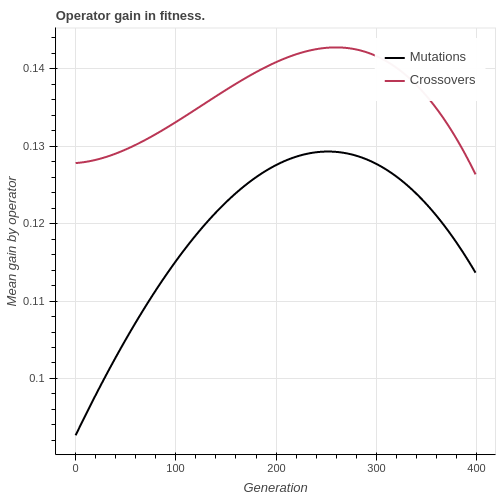
\includegraphics[width=0.8\linewidth]{figures/coolinggain.png}
        \caption{Mutation gain with cooling schedule.}
    \end{subfigure}%
    \begin{subfigure}{0.6\textwidth}
    \centering
        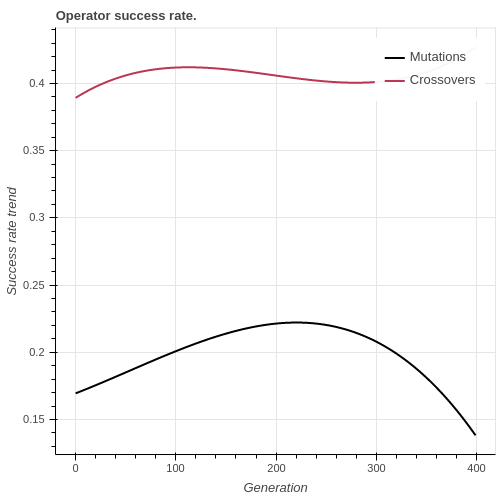
\includegraphics[width=0.8\linewidth]{figures/coolingrate.png}
        \caption{Mutation success rate with cooling schedule.}
    \end{subfigure}
        \begin{subfigure}{0.6\textwidth}
    \centering
        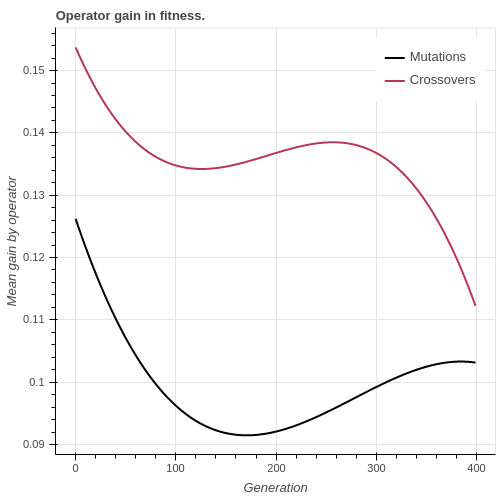
\includegraphics[width=0.8\linewidth]{figures/noncoolinggain.png}
        \caption{Mutation gain without cooling schedule.}
    \end{subfigure}%
    \begin{subfigure}{0.6\textwidth}
    \centering
        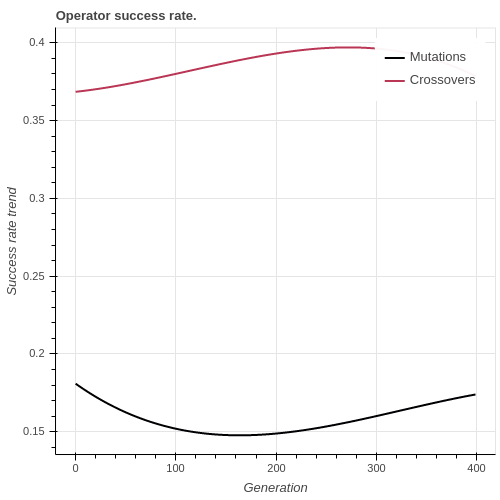
\includegraphics[width=0.8\linewidth]{figures/noncoolingrate.png}
        \caption{Mutation success rate without cooling schedule.}
    \end{subfigure}
    \caption{Effect of cooling schedule on mutation success rate and gain.}
    \label{fig:cooling}
    \end{figure}
In Figure \ref{fig:cooling} we see that both the success rate and gain for mutation are significantly higher over the generations when we apply the cooling schedule. In the final generations we see that without cooling the mutation success rate start to increase slightly, whereas with cooling it sharply decreases. This could indicate that the schedule is no longer effective in the final stages of the algorithm. This demonstrates that the schedule is only a heuristic, it attempts to emulate the knowledge needed in order to justify a mutation.
%\subsubsection{Depth sensitive}


% Exclusive experiments
\subsection{Constant Folding}\label{subsecfoldingresults}
\subsubsection{Savings}
We will analyze the results of our constant subtree folding technique discussed in section \ref{secconstfolding}.
\paragraph{Configuration}
\begin{itemize}
\item population : 20
\item minimum depth : 4
\item maximum depth : 10
\item phases : 20
\item generations per phase : 20
\item datapoints : 20
\item range : [1,5]
\item features : 5
\item archivesize : 20
\item expressions to archive per phase : 4
\item optimization strategy : none
\item testproblem : 1
\end{itemize}
The results for constant folding are similar for all testproblems, we select a single problem in order to visualize the constant folding  process over time instead of reporting only the results at the end.
% Figure
\begin{figure}
    \centering
    \begin{subfigure}{0.6\textwidth}
    \centering
        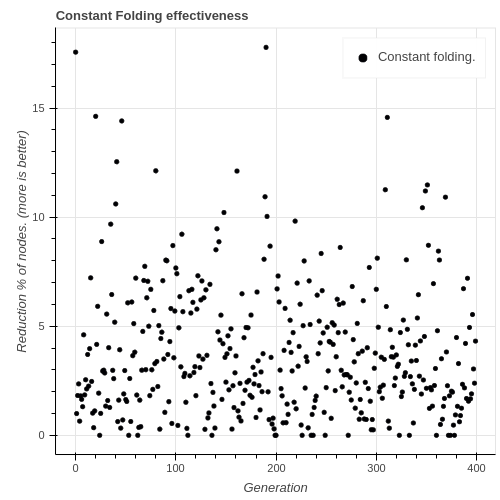
\includegraphics[width=0.8\linewidth]{figures/ctfold.png}
        \caption{Folding savings over generations.}
    \end{subfigure}%
    \begin{subfigure}{0.6\textwidth}
    \centering
        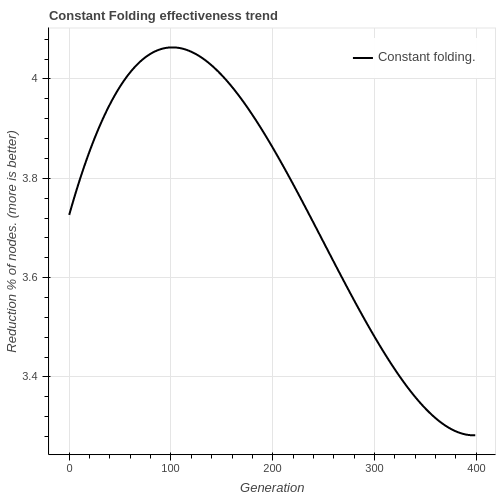
\includegraphics[width=0.8\linewidth]{figures/ctfoldtrend.png}
        \caption{Folding savings trend over generations (cubic fit).}
    \end{subfigure}
    \caption{Constant subtree folding savings over generations for testproblem 1.}
    \label{fig:ctfoldproblem1}
    \end{figure}
\paragraph{Discussion}
\subparagraph{Measure}
If we can collapse j subtrees holding $k_j$ nodes in a tree with n nodes, we define the savings as 
\[
s = \frac{\sum_{i=0}^{j} k_i - 1}{n} * 100
\]
In other words, s is the percentage of nodes with which a tree is reduced in size.
We calculate the mean for the entire generation of this value.
In Figure \ref{fig:ctfoldproblem1} we see that the savings have a high variance, but tend to decrease slightly. On average we expect between 1 and 5 \% in savings. In addition to the savings these results give us an indication as to how the algorithm introduces constant subtrees. If we would not apply the savings we would see an incremental gain in constant subtrees. Even though the gains are relatively small the high number of generations would make this tendency problematic. 
Constant folding prevents this from occurring, but as we have discussed previously it can also hinder convergence by slowing down the search process for the 'right' constant. Even though a constant subtree can be represented by a single constant, it holds more information than that single constant alone and provides a kind of 'constant repository' that can be used by the operators to more quickly find fitter expressions. On the other hand if the constant subtrees grow so large as to dominate the tree the convergence can be compromised as the tree has no more place left for base functions using features. A delicate balance between the two is required here. In future work we could experiment with such a balance by delaying the constant folding until x generations have passed, instead of our current approach where we apply it after every generation. 
% add to future work.

\subsection{Constant optimization}\label{subsec:optimizers}
We look at the effect constant optimization using different algorithms has on different configurations of the tool. The measures used in the comparison are best fitness on training and test data, mean fitness on training and test data, and optimization cost.

\subsubsection{Test problem}
To verify our implementation for the optimizers we use a simple test problem and observe for each optimizer if it is able to optimize this instance to a known optimal value.
\[
f(x_0, x_1, x_2) = 1 + x_1 * \sin (5+x_2) * x_0 + (17 + \sin (233+9))
\]
We give each optimizer a population of 50, 50 iterations and compare the results for 10 runs, displaying best value obtained, mean, and standard deviation of the fitness values compared to the known best value.
\paragraph{Best fitness}
In Figure \ref{fig:testproblembest} we see that DE outperforms PSO and ABC with several orders of magnitude. The best fitness value obtained was 2.22 e-16. As smaller but significant difference is present between PSO and ABC. This result is somewhat surprising given that fact that ABC is allowed to perform more evaluations in its configuration. From our previous discussion \ref{psocost},\ref{decost},\ref{abccost} we can conclude that for this test problem DE is clearly preferable as it obtains the best result at minimum cost. ABC has almost double the cost compared to PSO and DE, with PSO and DE having an equal cost in evaluations. The results on this testproblem do not necessarily mean that in the application of the three optimizers the results will be identical. Here we have a known optimal solution and want to observe how fast the optimizers converge to it. When we optimize evolved expressions we do not know what the optimal solution is. The problem statement is different, and so the convergence behavior is likely to differ as well. 
\paragraph{Distribution of fitness}
In Figures \ref{fig:testproblemmean} and \ref{fig:testproblemsd} we see that both the mean and standard deviation follow the same pattern as seen for the minimum fitness value with DE leading the others by several orders of magnitude. With all three distributions behaving similarly, this result provides a more solid foundation for our conclusions that for this problem DE is indeed the better optimizer.
\begin{figure}
    \centering
    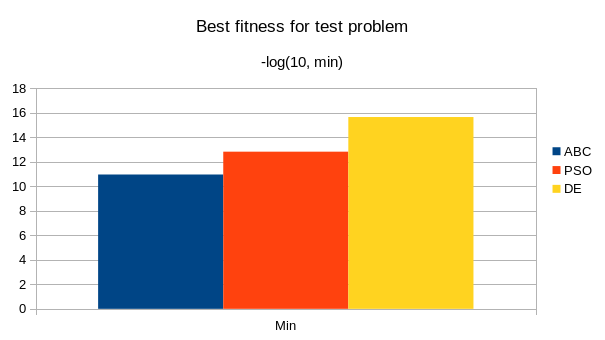
\includegraphics[width=\textwidth,height=\textheight,keepaspectratio]{figures/testproblem_bestfitness.png}
    \caption{Logarithmic value of best fitness for each optimizer.}
    \label{fig:testproblembest}
\end{figure}
\begin{figure}
    \centering
    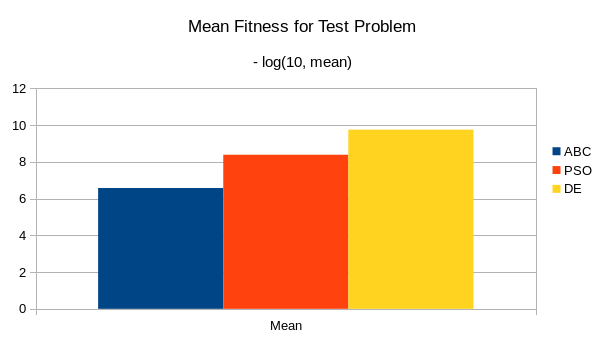
\includegraphics[width=\textwidth,height=\textheight,keepaspectratio]{figures/testproblem_meanfitness.png}
    \caption{Logarithmic scaled mean fitness for each optimizer.}
    \label{fig:testproblemmean}
\end{figure}
\begin{figure}
    \centering
    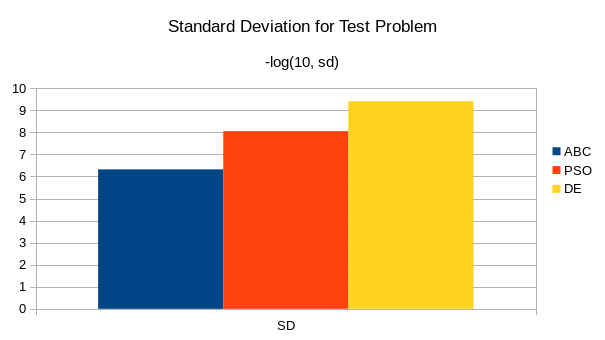
\includegraphics[width=\textwidth,height=\textheight,keepaspectratio]{figures/testproblem_sdfitness.png}
    \caption{Logarithmic scaled standard deviation fitness for each optimizer.}
    \label{fig:testproblemsd}
\end{figure}

\subsubsection{Optimizer experiments setup}
We test the 15 expressions with the following configuration:
\begin{itemize}
\item population : 20
\item minimum depth : 4
\item maximum depth : 10
\item phases : (2, 5, 10)
\item generations per phase : 20
\item datapoints : 20
\item range : [1,5]
\item features : 5
\item archivesize : 20
\item expressions to archive per phase : 4
\item optimization strategy : optimize expressions archived at end of phase
\end{itemize}
\subsubsection{Measures}
We compare the relative gain in fitness compared to not using an optimizer for all expressions. 
In other words, if $m_n$ is a measure obtained by the algorithm without the optimizer, and $m_a$ the same measure with the optimizer, we then define the relative gain as :
\[
g_{ma} = \frac{m_n}{m_a}
\]
If $m_a$ is zero, we use $-log_{10}(m_n)$ to represent the gain. If both are zero, the gain is obviously 1. A value of g $>$ 1 indicates the ratio with which the optimizer improves the result. A g value $<$ 1 indicates a regression.
These 15 functions have wildly varying convergence behavior. In order to make sense of the data, we then apply a log scale :
\[
g_{lma} = - \log_{10}(g_{ma})
\]
A value of $g_{lma} > 0 $ indicates improvement, with the units transformed to orders of magnitude. A zero value indicates no improvement is registered, and negative values indicate regression. 
As measures we use the best fitness value on the training data, and the best on the full data set. We take the mean of the fitness of the 5 best expressions on training and the full data as well. This last measure gives us an indication on how the optimization process acts on the 'best' set of the population. Note that in our configuration, the 4 best expressions are always optimized.
\subsubsection{2 Phases}
In Figure \ref{fig:2phase} we see the performance of the algorithms on training data. 
In Table \ref{table:2phasemintrain} we see that for problems 0, 4, 5 there is no improvement possible (e.g. zero fitness value), which explains the absence of any value in the figure.
We see that for the training fitness data the improvements are significant, with ABC scoring an increase of 2.5 orders of magnitude for problem 6. For the other problems the increase is still large, especially given that our fitness function has a range of [0,1].
We also observe the significant regression for problem 6. This is likely caused due to overfitting. The algorithm in question (DE) optimizes the 4 best candidates of the last phase, but it is possible that these optimized expressions actually form a local optimum for the training data which has poor fitness values for the validation data. By archiving these the convergence of the algorithm is hindered in the next phase. Note that DE allows equality updates, where expressions with the same fitness values are accepted as better. The same behavior occurs in a far less significant effect for expressions 7 and 9. A second explanation is our implementation of the population. The algorithm enforces distinct fitness values for all expressions. In an edge case it is possible that these optimized samples form a barrier, preventing other expressions from evolving past them. The optimized expressions in effect trap the rest of the population, which given our low generation count can explain this behavior.
The mean fitness of the 5 best expressions shows significant improvements. Important to observe is the similarity between the two plots, the correlation between fitness values on training and full data is strong. This was a concern in the setup of the experiments. The optimizers could introduce overfitting on the training data. This risk is mitigated by the relatively low number of iterations each optimizer has been allocated.
For the minimum fitness on the full data ABC outperforms the others. For the mean evaluation PSO is a good candidate. In this stage of the experiments, there is no single algorithm that is ideal for all problems. This once again confirms the NFL theorem \cite{NFL}.

% Figures
\begin{figure}
    \centering
    \begin{subfigure}{0.6\textwidth}
    \centering
        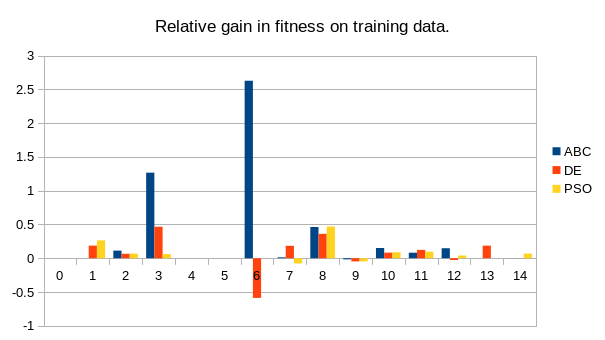
\includegraphics[width=0.8\linewidth]{figures/hybrid_phases2_mintrainfitness.png}
        \caption{Relative gain in best fitness of training data}
    \end{subfigure}%
    \begin{subfigure}{0.6\textwidth}
    \centering
        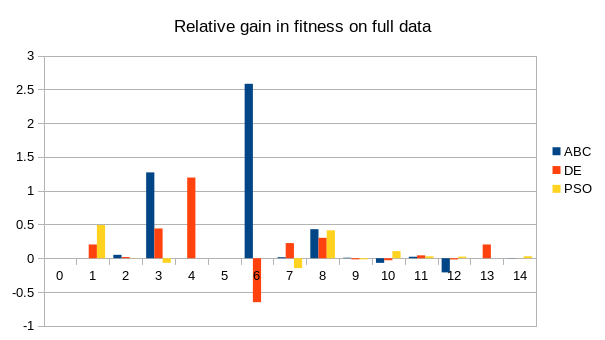
\includegraphics[width=0.8\linewidth]{figures/hybrid_phases2_minfullfitness.png}
        \caption{Relative gain in best fitness of full data}
    \end{subfigure}
        \begin{subfigure}{0.6\textwidth}
    \centering
        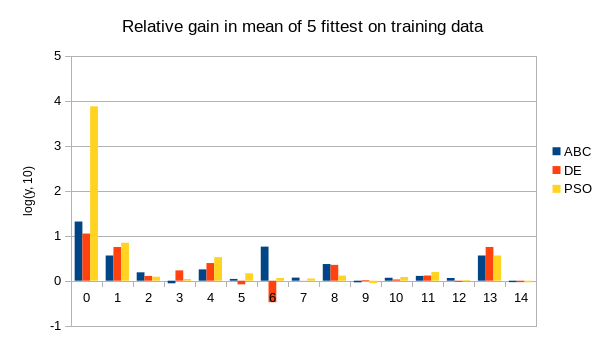
\includegraphics[width=0.8\linewidth]{figures/hybrid_phases2_meantrainfitness.png}
        \caption{Relative gain in mean fitness of training data}
    \end{subfigure}%
    \begin{subfigure}{0.6\textwidth}
    \centering
        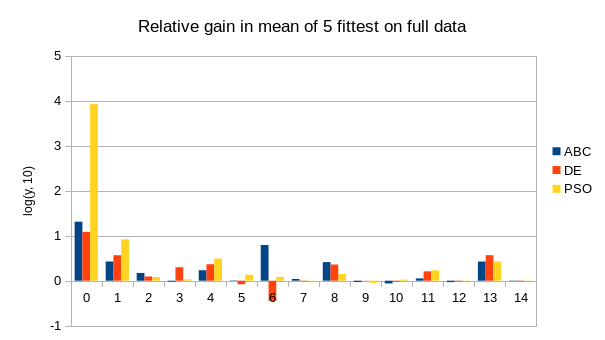
\includegraphics[width=0.8\linewidth]{figures/hybrid_phases2_meanfullfitness.png}
        \caption{Relative gain in mean fitness of full data}
    \end{subfigure}
    \caption{Relative gain of optimizer after 2 phases.}
    \label{fig:2phase}
    \end{figure}

% Table
\begin{landscape}
\begin{table}[]
\centering
\caption{Relative Gain in minimum fitness on training data after 2 phases.}
\label{table:2phasemintrain}
\begin{adjustbox}{width=1.7\textwidth}
\begin{tabular}{lllllllllllllllll}
          &           &           &           &           &           &           &           &           &           &           &           &           &           &           &           &  \\
           & 0         & 1         & 2         & 3         & 4         & 5         & 6         & 7         & 8         & 9         & 10        & 11        & 12        & 13        & 14        &  \\
ABC                 & 1.000e+00 & 1.000e+00 & 1.295e+00 & 1.848e+01 & 1.000e+00 & 1.000e+00 & 4.253e+02 & 1.030e+00 & 2.897e+00 & 9.615e-01 & 1.415e+00 & 1.207e+00 & 1.404e+00 & 1.000e+00 & 9.970e-01 &  \\
DE                  & 1.000e+00 & 1.536e+00 & 1.163e+00 & 2.923e+00 & 1.000e+00 & 1.000e+00 & 2.584e-01 & 1.526e+00 & 2.294e+00 & 8.972e-01 & 1.210e+00 & 1.327e+00 & 9.397e-01 & 1.536e+00 & 9.960e-01 &  \\
PSO                 & 1.000e+00 & 1.839e+00 & 1.169e+00 & 1.150e+00 & 1.000e+00 & 1.000e+00 & 1.000e+00 & 8.356e-01 & 2.947e+00 & 8.971e-01 & 1.226e+00 & 1.247e+00 & 1.096e+00 & 1.000e+00 & 1.172e+00 &  \\

\end{tabular}
\end{adjustbox}
\end{table}

\begin{table}[]
\centering
\caption{Gain in minimum fitness on full data after 2 phases.}
\label{table:2phaseminfull}
\begin{adjustbox}{width=1.7\textwidth}
\begin{tabular}{lllllllllllllllll}
         &           &           &           &           &           &           &           &           &           &           &           &           &           &           &           &  \\
         & 0         & 1         & 2         & 3         & 4         & 5         & 6         & 7         & 8         & 9         & 10        & 11        & 12        & 13        & 14        &  \\
ABC                 & 1.000e+00 & 1.000e+00 & 1.122e+00 & 1.865e+01 & 1.000e+00 & 1.000e+00 & 3.831e+02 & 1.034e+00 & 2.691e+00 & 1.016e+00 & 8.528e-01 & 1.051e+00 & 6.169e-01 & 1.000e+00 & 9.938e-01 &  \\
DE                  & 1.000e+00 & 1.597e+00 & 1.039e+00 & 2.757e+00 & 1.565e+01 & 1.000e+00 & 2.233e-01 & 1.674e+00 & 2.004e+00 & 9.617e-01 & 9.337e-01 & 1.103e+00 & 9.584e-01 & 1.597e+00 & 9.970e-01 &  \\
PSO                 & 1.000e+00 & 3.098e+00 & 9.915e-01 & 8.538e-01 & 1.000e+00 & 1.000e+00 & 1.000e+00 & 7.145e-01 & 2.586e+00 & 9.617e-01 & 1.274e+00 & 1.067e+00 & 1.055e+00 & 1.000e+00 & 1.069e+00 &  \\
\end{tabular}
\end{adjustbox}
\end{table}

\begin{table}[]
\centering
\caption{Relative gain in mean fitness of 5 fittest expressions on training data after 2 phases.}
\label{table:2phasemeantrain}
\begin{adjustbox}{width=1.7\textwidth}
\begin{tabular}{lllllllllllllllll}
&           &           &           &           &           &           &           &           &           &           &           &           &           &           &           &  \\
           & 0         & 1         & 2         & 3         & 4         & 5         & 6         & 7         & 8         & 9         & 10        & 11        & 12        & 13        & 14        &  \\
ABC                 & 1.335e+01 & 1.113e+00 & 4.824e+00 & 5.543e-01 & 3.479e+02 & 4.395e+02 & 7.059e-02 & 4.477e-01 & 1.215e+00 & 9.073e-01 & 2.214e+00 & 9.169e-01 & 1.564e+00 & 1.113e+00 & 4.064e-01 &  \\
DE                  & 3.620e+01 & 1.299e+00 & 1.115e+00 & 1.128e+00 & 1.204e-01 & 5.385e+08 & 3.202e+01 & 1.338e+00 & 1.835e+00 & 1.154e+00 & 1.268e+00 & 1.626e+00 & 1.246e+00 & 1.299e+00 & 7.247e-01 &  \\
PSO                 & 5.046e+02 & 8.017e+00 & 2.302e+00 & 4.220e-01 & 1.665e+01 & 2.237e+01 & 2.144e-01 & 6.974e-01 & 1.240e+00 & 9.647e-01 & 1.408e+00 & 1.347e+00 & 5.933e+00 & 7.152e-01 & 8.523e-01 &  \\


\end{tabular}
\end{adjustbox}
\end{table}


\begin{table}[]
\centering
\caption{Relative gain in mean fitness of 5 fittest expressions on full data after 2 phases.}
\label{table:2phasemeanfull}
\begin{adjustbox}{width=1.7\textwidth}
\begin{tabular}{lllllllllllllllll}
      &           &           &           &           &           &           &           &           &           &           &           &           &           &           &           &  \\
algorithm           & 0         & 1         & 2         & 3         & 4         & 5         & 6         & 7         & 8         & 9         & 10        & 11        & 12        & 13        & 14        &  \\
ABC                 & 1.382e+01 & 2.306e-01 & 5.950e+00 & 5.551e-01 & 3.264e+02 & 5.091e+02 & 7.308e-02 & 4.463e-01 & 1.188e+00 & 9.214e-01 & 4.665e-01 & 7.197e-01 & 1.463e+00 & 2.306e-01 & 8.096e-01 &  \\
DE                  & 3.244e+01 & 1.315e+00 & 1.068e+00 & 1.228e+00 & 1.153e-01 & 5.392e+08 & 3.234e+01 & 1.348e+00 & 1.685e+00 & 1.153e+00 & 1.193e+00 & 1.441e+00 & 1.210e+00 & 1.315e+00 & 1.199e+00 &  \\
PSO                 & 4.920e+02 & 6.794e+00 & 2.531e+00 & 4.117e-01 & 1.721e+01 & 9.994e+00 & 2.146e-01 & 6.486e-01 & 1.113e+00 & 7.060e-01 & 5.830e-01 & 1.324e+00 & 2.613e+00 & 8.126e-01 & 1.094e+00 & \\

\end{tabular}
\end{adjustbox}
\end{table}
\end{landscape}



\subsubsection{5 Phases}
With 5 phases we see in Figure\ref{fig:5phase} a more diverse effect. While ABC scores exceptionally good on problem 6, in sharp contrast with the 2 phase experiment, we see that PSO scores overall better for the training data. These results are logarithmic scaled, an improvement in fitness of factor 10 results in a value of 1 in the plots. When it comes to improving the mean of the best 5 expressions, PSO is a stable choice if we disregard the outlier values for problem 5. The correlation between training and full fitness scores is good for both measures. This demonstrates that the optimizer is not in this experiment introducing overfitting on the training data. The adverse effect of the optimizer on some test problems is still present.
For the best fitness values on the full data DE is the better candidate. While ABC scores exceptionally high on problem 6, DE scores better overall. When we look at the mean there is no clear winner. 
\begin{figure}
    \centering
    \begin{subfigure}{0.6\textwidth}
    \centering
        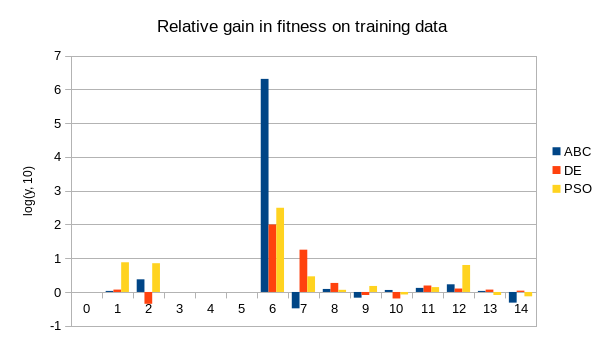
\includegraphics[width=0.8\linewidth]{figures/hybrid_phases5_mintrainfitness.png}
        \caption{Relative gain in best fitness of training data}
    \end{subfigure}%
    \begin{subfigure}{0.6\textwidth}
    \centering
        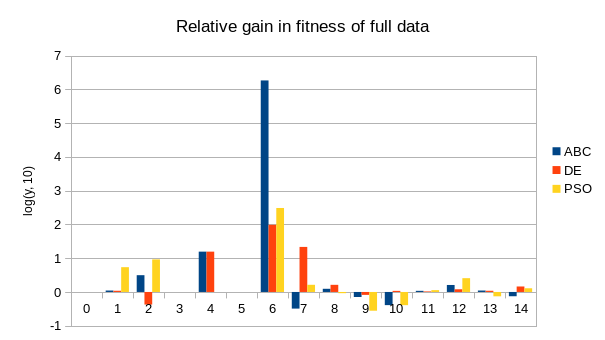
\includegraphics[width=0.8\linewidth]{figures/hybrid_phases5_minfullfitness.png}
        \caption{Relative gain in best fitness of full data}
    \end{subfigure}
        \begin{subfigure}{0.6\textwidth}
    \centering
        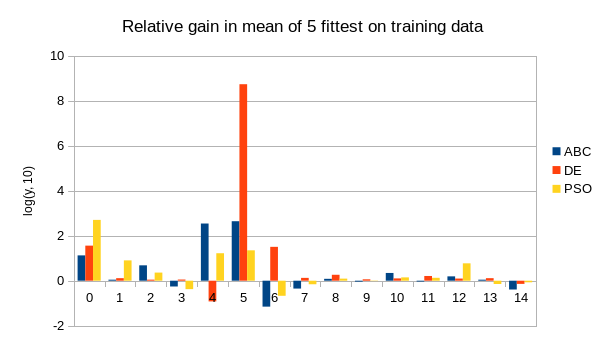
\includegraphics[width=0.8\linewidth]{figures/hybrid_phases5_meantrainfitness.png}
        \caption{Relative gain in mean fitness of training data}
    \end{subfigure}%
    \begin{subfigure}{0.6\textwidth}
    \centering
        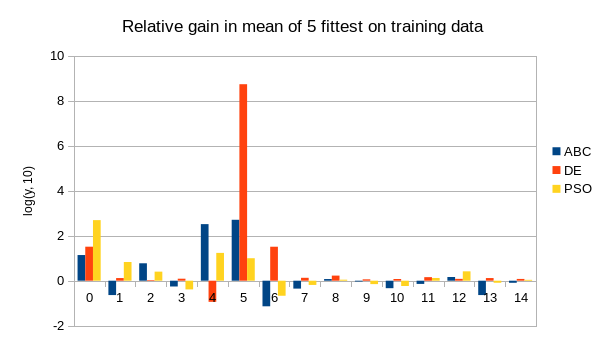
\includegraphics[width=0.8\linewidth]{figures/hybrid_phases5_meanfullfitness.png}
        \caption{Relative gain in mean fitness of full data}
    \end{subfigure}
    \caption{Relative gain of optimizer after 5 phases.}
    \label{fig:5phase}
    \end{figure}

% Table
\begin{landscape}
\begin{table}[]
\centering
\caption{Relative Gain in minimum fitness on training data after 5 phases.}
\label{table:5phasemintrain}
\begin{adjustbox}{width=1.7\textwidth}
\begin{tabular}{lllllllllllllllll}
     &           &           &           &           &           &           &           &           &           &           &           &           &           &           &           &  \\
algorithm           & 0         & 1         & 2         & 3         & 4         & 5         & 6         & 7         & 8         & 9         & 10        & 11        & 12        & 13        & 14        &  \\
ABC                 & 1.000e+00 & 1.074e+00 & 2.371e+00 & 1.000e+00 & 1.000e+00 & 1.000e+00 & 2.050e+06 & 3.277e-01 & 1.230e+00 & 6.779e-01 & 1.146e+00 & 1.321e+00 & 1.690e+00 & 1.074e+00 & 4.837e-01 &  \\
DE                  & 1.000e+00 & 1.176e+00 & 4.459e-01 & 1.000e+00 & 1.000e+00 & 1.000e+00 & 9.987e+01 & 1.790e+01 & 1.853e+00 & 8.129e-01 & 6.428e-01 & 1.553e+00 & 1.266e+00 & 1.176e+00 & 1.095e+00 &  \\
PSO                 & 1.000e+00 & 7.591e+00 & 7.112e+00 & 0.000e+00 & 1.000e+00 & 1.000e+00 & 3.117e+02 & 2.904e+00 & 1.159e+00 & 1.506e+00 & 8.442e-01 & 1.396e+00 & 6.302e+00 & 8.146e-01 & 7.435e-01 &  \\

\end{tabular}
\end{adjustbox}
\end{table}

\begin{table}[]
\centering
\caption{Gain in minimum fitness on full data after 5 phases.}
\label{table:5phaseminfull}
\begin{adjustbox}{width=1.7\textwidth}
\begin{tabular}{lllllllllllllllll}
            &           &           &           &           &           &           &           &           &           &           &           &           &           &           &           &  \\
           & 0         & 1         & 2         & 3         & 4         & 5         & 6         & 7         & 8         & 9         & 10        & 11        & 12        & 13        & 14        &  \\
ABC                 & 1.000e+00 & 1.103e+00 & 3.145e+00 & 1.000e+00 & 1.565e+01 & 1.000e+00 & 1.846e+06 & 3.220e-01 & 1.243e+00 & 7.106e-01 & 4.082e-01 & 1.080e+00 & 1.613e+00 & 1.103e+00 & 7.483e-01 &  \\
DE                  & 1.000e+00 & 1.087e+00 & 4.240e-01 & 1.000e+00 & 1.565e+01 & 1.000e+00 & 9.756e+01 & 2.158e+01 & 1.629e+00 & 8.213e-01 & 1.079e+00 & 1.040e+00 & 1.202e+00 & 1.087e+00 & 1.454e+00 &  \\
PSO                 & 1.000e+00 & 5.426e+00 & 9.234e+00 & 0.000e+00 & 1.000e+00 & 1.000e+00 & 3.070e+02 & 1.634e+00 & 9.216e-01 & 2.786e-01 & 4.071e-01 & 1.131e+00 & 2.563e+00 & 7.444e-01 & 1.288e+00 &  \\

\end{tabular}
\end{adjustbox}
\end{table}

\begin{table}[]
\centering
\caption{Relative gain in mean fitness of 5 fittest expressions on training data after 5 phases.}
\label{table:5phasemeantrain}
\begin{adjustbox}{width=1.7\textwidth}
\begin{tabular}{lllllllllllllllll}
 &           &           &           &           &           &           &           &           &           &           &           &           &           &           &           &  \\
           & 0         & 1         & 2         & 3         & 4         & 5         & 6         & 7         & 8         & 9         & 10        & 11        & 12        & 13        & 14        &  \\
ABC                 & 2.064e+01 & 3.632e+00 & 1.536e+00 & 8.774e-01 & 1.788e+00 & 1.096e+00 & 5.726e+00 & 1.173e+00 & 2.348e+00 & 9.209e-01 & 1.163e+00 & 1.280e+00 & 1.151e+00 & 3.632e+00 & 9.300e-01 &  \\
DE                  & 1.117e+01 & 5.624e+00 & 1.277e+00 & 1.696e+00 & 2.468e+00 & 8.307e-01 & 3.333e-01 & 9.953e-01 & 2.249e+00 & 1.038e+00 & 1.067e+00 & 1.305e+00 & 9.416e-01 & 5.624e+00 & 9.302e-01 &  \\
PSO                 & 7.494e+03 & 6.977e+00 & 1.225e+00 & 1.091e+00 & 3.335e+00 & 1.461e+00 & 1.154e+00 & 1.118e+00 & 1.300e+00 & 8.794e-01 & 1.212e+00 & 1.559e+00 & 1.041e+00 & 3.632e+00 & 9.242e-01 &  \\

\end{tabular}
\end{adjustbox}
\end{table}


\begin{table}[]
\centering
\caption{Relative gain in mean fitness of 5 fittest expressions on full data after 5 phases.}
\label{table:5phasemeanfull}
\begin{adjustbox}{width=1.7\textwidth}
\begin{tabular}{lllllllllllllllll}
    &           &           &           &           &           &           &           &           &           &           &           &           &           &           &           &  \\
    & 0         & 1         & 2         & 3         & 4         & 5         & 6         & 7         & 8         & 9         & 10        & 11        & 12        & 13        & 14        &  \\
ABC                 & 2.048e+01 & 2.672e+00 & 1.487e+00 & 9.516e-01 & 1.709e+00 & 1.021e+00 & 6.217e+00 & 1.093e+00 & 2.589e+00 & 9.346e-01 & 8.686e-01 & 1.126e+00 & 9.308e-01 & 2.672e+00 & 9.816e-01 &  \\
DE                  & 1.213e+01 & 3.687e+00 & 1.244e+00 & 1.997e+00 & 2.324e+00 & 8.352e-01 & 3.572e-01 & 9.731e-01 & 2.288e+00 & 1.009e+00 & 9.496e-01 & 1.616e+00 & 9.641e-01 & 3.687e+00 & 9.668e-01 &  \\
PSO                 & 8.382e+03 & 8.286e+00 & 1.204e+00 & 1.071e+00 & 3.111e+00 & 1.362e+00 & 1.219e+00 & 9.817e-01 & 1.411e+00 & 8.939e-01 & 1.059e+00 & 1.698e+00 & 1.018e+00 & 2.672e+00 & 9.840e-01 & 

\end{tabular}
\end{adjustbox}
\end{table}
\end{landscape}

\subsubsection{10 Phases}
If we observe the convergence after 10 phases we see a more pronounced effect. In Figure \ref{fig:10phase} we see that for several problems the optimizers are no longer improving w.r.t the unoptimized algorithm. This only holds for the best values, for the mean values the improvements are still significant. It becomes clear that the optimizer can force the algorithm into a local optimum from which it becomes hard to escape. The correlation between fitness results on the training data and full data is starting to weaken as well, in comparison to the experiments with 2 and 5 phases. 
If we look at the fitness values for the full data DE is the more stable of the three algorithms. When it regresses its losses are smaller than the others, while its gains are strongest on the most problems. For the mean fitness of the full data a similar argument can be made, with the exception of problem 2 where DE fails severely.
Another aspect is that after 100 generations the fitness values are extremely small, in the order of 1e-15. We measure the relative gain with respect to the algorithm without an optimizer, but as the fitness values decrease rounding errors start to influence the calculations more and more. The fitness values are approaching the floating point epsilon values. For our implementation epsilon is set at 2.22 e-16. For problem 0, a minimum fitness value of 0 is found after 2 phases. For others far more iterations are needed. We need to make a trade-off in order to be able to compare all 15 problems. Giving each problem an equal budget in iterations is the more fair approach. Another approach is implementing a stop condition that halts within a certain distance of a desired fitness treshold, but this approach is fraught with issues. There is no guarantee exactly how many iterations are needed. This approach requires knowing the problem 'hardness' in advance, but by the very definition of our problem statement we do not know how hard our problem is. We do not know the optimal value, or even if there is a singular optimal value. In general the topology of the search space SR tries to traverse is not known. A practitioner with a real world problem faces the same issues. A more robust approach is stating in advance how much resources the algorithm can use in its search, and terminate if that budget is exhausted. The exact definition of resource is nuanced. We can use time, but this depends to a large extent on the implementation. A more solid measure is the number of fitness evaluations. Even this is not a constant measure, not all evaluations are equal in computational complexity.
\begin{figure}
    \centering
    \begin{subfigure}{0.6\textwidth}
    \centering
        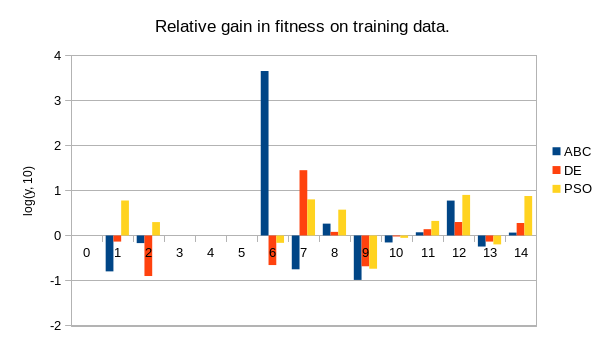
\includegraphics[width=0.8\linewidth]{figures/hybrid_phases10_mintrainfitness.png}
        \caption{Relative gain in best fitness of training data}
    \end{subfigure}%
    \begin{subfigure}{0.6\textwidth}
    \centering
        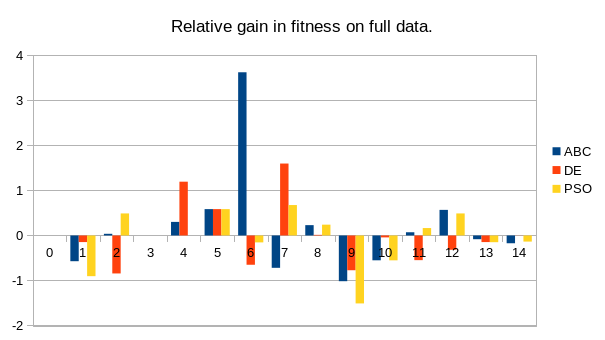
\includegraphics[width=0.8\linewidth]{figures/hybrid_phases10_minfullfitness.png}
        \caption{Relative gain in best fitness of full data}
    \end{subfigure}
        \begin{subfigure}{0.6\textwidth}
    \centering
        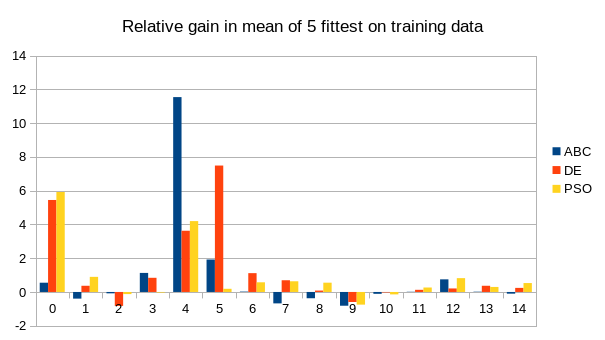
\includegraphics[width=0.8\linewidth]{figures/hybrid_phases10_meantrainfitness.png}
        \caption{Relative gain in mean fitness of training data}
    \end{subfigure}%
    \begin{subfigure}{0.6\textwidth}
    \centering
        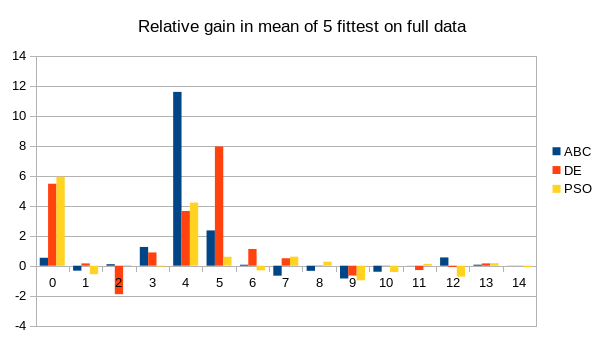
\includegraphics[width=0.8\linewidth]{figures/hybrid_phases10_meanfullfitness.png}
        \caption{Relative gain in mean fitness of full data}
    \end{subfigure}
    \caption{Relative gain of optimizer after 10 phases.}
    \label{fig:10phase}
    \end{figure}

% Table
\begin{landscape}
\begin{table}[]
\centering
\caption{Relative Gain in minimum fitness on training data after 10 phases.}
\label{table:10phasemintrain}
\begin{adjustbox}{width=1.7\textwidth}
\begin{tabular}{lllllllllllllllll}
     &           &           &           &           &           &           &           &           &           &           &           &           &           &           &           &  \\
 & 0         & 1         & 2         & 3         & 4         & 5         & 6         & 7         & 8         & 9         & 10        & 11        & 12        & 13        & 14        &  \\
ABC                 & 1.000e+00 & 1.591e-01 & 6.759e-01 & 1.000e+00 & 1.000e+00 & 1.000e+00 & 4.508e+03 & 1.771e-01 & 1.831e+00 & 1.029e-01 & 6.983e-01 & 1.176e+00 & 5.945e+00 & 5.674e-01 & 1.158e+00 &  \\
DE                  & 1.000e+00 & 7.304e-01 & 1.254e-01 & 1.000e+00 & 1.000e+00 & 1.000e+00 & 2.197e-01 & 2.816e+01 & 1.201e+00 & 2.068e-01 & 9.480e-01 & 1.377e+00 & 1.989e+00 & 7.304e-01 & 1.891e+00 &  \\
PSO                 & 1.000e+00 & 5.976e+00 & 1.980e+00 & 1.000e+00 & 1.000e+00 & 1.000e+00 & 6.857e-01 & 6.335e+00 & 3.739e+00 & 1.822e-01 & 8.852e-01 & 2.105e+00 & 7.945e+00 & 6.334e-01 & 7.526e+00 &  \\

\end{tabular}
\end{adjustbox}
\end{table}

\begin{table}[]
\centering
\caption{Gain in minimum fitness on full data after 10 phases.}
\label{table:10phaseminfull}
\begin{adjustbox}{width=1.7\textwidth}
\begin{tabular}{lllllllllllllllll}
         &           &           &           &           &           &           &           &           &           &           &           &           &           &           &           &  \\
         & 0         & 1         & 2         & 3         & 4         & 5         & 6         & 7         & 8         & 9         & 10        & 11        & 12        & 13        & 14        &  \\
ABC                 & 1.000e+00 & 2.679e-01 & 1.087e+00 & 1.000e+00 & 2.000e+00 & 3.846e+00 & 4.224e+03 & 1.908e-01 & 1.694e+00 & 9.627e-02 & 2.807e-01 & 1.178e+00 & 3.699e+00 & 8.255e-01 & 6.709e-01 &  \\
DE                  & 1.000e+00 & 7.126e-01 & 1.432e-01 & 1.000e+00 & 1.565e+01 & 3.846e+00 & 2.232e-01 & 3.965e+01 & 1.031e+00 & 1.687e-01 & 9.052e-01 & 2.827e-01 & 4.813e-01 & 7.126e-01 & 1.005e+00 &  \\
PSO                 & 1.000e+00 & 1.246e-01 & 3.083e+00 & 1.000e+00 & 1.000e+00 & 3.846e+00 & 7.019e-01 & 4.738e+00 & 1.736e+00 & 3.091e-02 & 2.797e-01 & 1.459e+00 & 3.081e+00 & 7.083e-01 & 7.305e-01 &  \\

\end{tabular}
\end{adjustbox}
\end{table}

\begin{table}[]
\centering
\caption{Relative gain in mean fitness of 5 fittest expressions on training data after 10 phases.}
\label{table:10phasemeantrain}
\begin{adjustbox}{width=1.7\textwidth}
\begin{tabular}{lllllllllllllllll}
 &           &           &           &           &           &           &           &           &           &           &           &           &           &           &           &  \\
 & 0         & 1         & 2         & 3         & 4         & 5         & 6         & 7         & 8         & 9         & 10        & 11        & 12        & 13        & 14        &  \\
ABC                 & 3.530e+00 & 4.032e-01 & 8.301e-01 & 1.346e+01 & 3.503e+11 & 8.400e+01 & 1.061e+00 & 2.112e-01 & 4.251e-01 & 1.531e-01 & 7.788e-01 & 1.034e+00 & 5.595e+00 & 1.041e+00 & 7.932e-01 &  \\
DE                  & 2.813e+05 & 2.333e+00 & 1.492e-01 & 6.914e+00 & 4.242e+03 & 3.098e+07 & 1.305e+01 & 4.957e+00 & 1.210e+00 & 2.547e-01 & 9.384e-01 & 1.339e+00 & 1.614e+00 & 2.333e+00 & 1.742e+00 &  \\
PSO                 & 8.346e+05 & 7.871e+00 & 7.495e-01 & 9.256e-01 & 1.573e+04 & 1.539e+00 & 3.743e+00 & 4.297e+00 & 3.560e+00 & 1.781e-01 & 7.192e-01 & 1.838e+00 & 6.612e+00 & 1.991e+00 & 3.372e+00 &  \\
\end{tabular}
\end{adjustbox}
\end{table}


\begin{table}[]
\centering
\caption{Relative gain in mean fitness of 5 fittest expressions on full data after 10 phases.}
\label{table:10phasemeanfull}
\begin{adjustbox}{width=1.7\textwidth}
\begin{tabular}{lllllllllllllllll}
     &           &           &           &           &           &           &           &           &           &           &           &           &           &           &           &  \\
     & 0         & 1         & 2         & 3         & 4         & 5         & 6         & 7         & 8         & 9         & 10        & 11        & 12        & 13        & 14        &  \\
ABC                 & 3.389e+00 & 4.674e-01 & 1.263e+00 & 1.779e+01 & 3.846e+11 & 2.257e+02 & 1.163e+00 & 2.171e-01 & 4.563e-01 & 1.408e-01 & 3.961e-01 & 1.020e+00 & 3.568e+00 & 1.170e+00 & 1.027e+00 &  \\
DE                  & 2.901e+05 & 1.426e+00 & 1.270e-02 & 7.677e+00 & 4.445e+03 & 8.874e+07 & 1.310e+01 & 3.143e+00 & 1.057e+00 & 2.200e-01 & 9.597e-01 & 5.134e-01 & 8.172e-01 & 1.426e+00 & 1.039e+00 &  \\
PSO                 & 8.487e+05 & 2.720e-01 & 1.113e+00 & 8.726e-01 & 1.601e+04 & 3.942e+00 & 4.913e-01 & 4.000e+00 & 1.855e+00 & 1.070e-01 & 3.816e-01 & 1.327e+00 & 1.873e-01 & 1.466e+00 & 8.262e-01 & 
\end{tabular}
\end{adjustbox}
\end{table}
\end{landscape}

\subsubsection{Cost}
The cost in terms of evaluations is linear in the number of phases. For each phase, 4 expressions are optimized with O(nk) complexity. In our configuration n=50, k=50. The SR algorithm itself requires O(mg) evaluations per phase, where m is the population (20) and g the generations per phase (20). The question whether or not the cost of the optimizer is worth the gain in fitness is in the end one for the practitioner to answer. There is no guarantee that improvement will take place, but from the results on the above hard problems we can still expect significant improvements up to several orders of magnitude.

\subsection{Distributed}
We now apply our tool to the testproblems in a distributed setup.

\subsubsection{Experiment setup}
\begin{itemize}
\item population : 20
\item minimum depth : 4
\item maximum depth : 8
\item phases : 20
\item generations per phase : 20
\item datapoints : 20
\item range : [1,5]
\item features : 5
\item archivesize : 20
\item expressions to archive per phase : 4
\item optimization strategy : none
\item communication size m : 2, 4
\item topology : Tree, Random, Grid
\item spreadpolicy : distribute
\item processes n : 25
\end{itemize}
\paragraph{Discussion}
From section \ref{subsec:commstrategies}
we know that simply using m for all topologies will lead to unintended communication patterns. We test Tree and Random with m = 2, and Grid with m = 4. This results in the following number of messages per link :
\begin{itemize}
\item Grid : 1
\item Tree : 1
\item Random : 2
\end{itemize}
The total number of messages sent per phase is then :
\begin{itemize}
\item Grid : 4 * n = 200
\item Tree : 1 * n = 25
\item Random : 2 * n = 50
\end{itemize}
The value of m = 2 for Tree and m = 4 for Grid follows from our discussion in \ref{subsec:commstrategies}. The Random topology in this configuration has a single outgoing link per process, resulting in 2 messages per link. This configuration forms a balance between the different strategies.
For 25 processes the grid topology is a simple square of 5x5. The tree topology with 25 processes is a non full binary tree with depth 4. The random topology is highly dependent on the seed. In Figure \ref{fig:experimenttopos} we see that in this instance the topology has become a disconnected graph of 3 cycles. This highlights the risk of using a random topology, without extra constraints the characteristics of the communication pattern are unknown and can be undesirable.
\begin{figure}
    \centering
    \begin{subfigure}{0.5\textwidth}
    \centering
        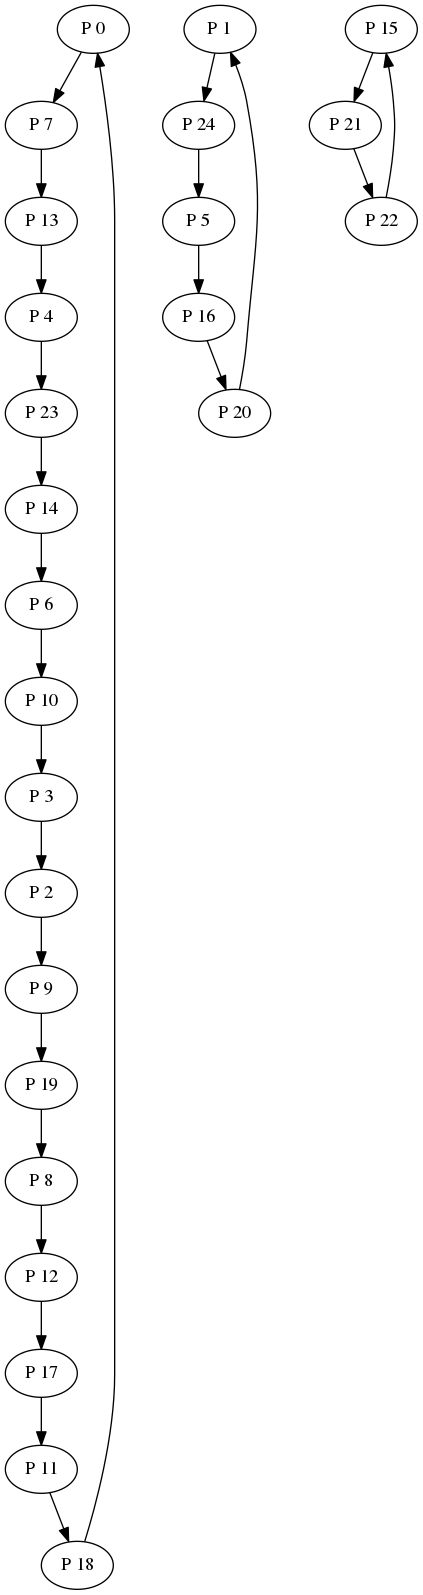
\includegraphics[width=0.5\linewidth]{figures/random25.png}
        \caption{Random topology for 25 processes with one outgoing link per process.}
    \end{subfigure}%
    \begin{subfigure}{0.5\textwidth}
    \centering
        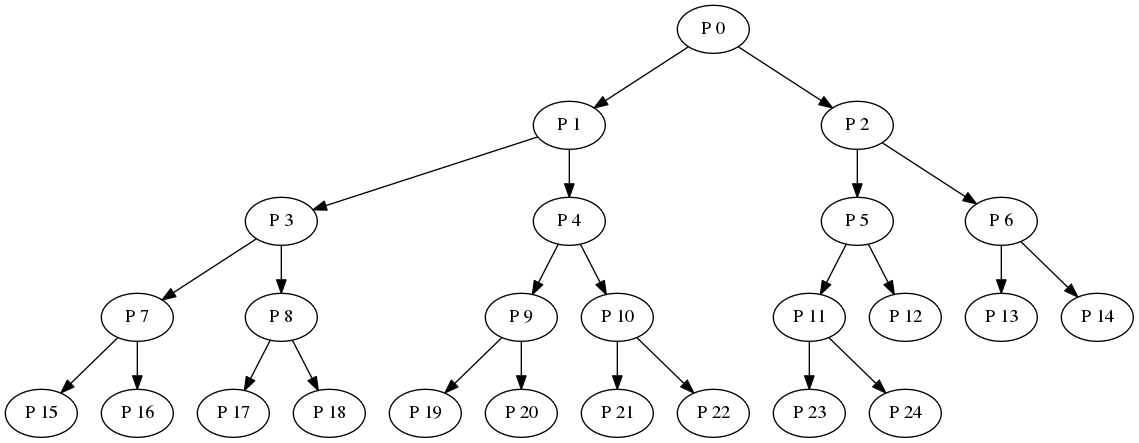
\includegraphics[width=0.5\linewidth]{figures/tree25.png}
        \caption{Tree topology for 25 processes.}
    \end{subfigure}
    \caption{Tree and random topologies used in the experiment.}
    \label{fig:experimenttopos}
    \end{figure}

\subsubsection{Measures}
When the experiment ends the best 20 expressions from all processes are collected and scored. We measure in best fitness on the training data, and best fitness on the validated data. As we have seen in % todo ref kfold 
there is a subtle difference here compared to the sequential approach. While each process has a subset of the training and validation data, in the end we score against the full dataset.
Finally we record the mean fitness values of the best 5 expressions, both on the training and validation data. These are the same measures as used by the optimizer experiment. The mean is restricted to the upper quarter of the population specifically to measure how the best expressions are distributed. This measure records the convergence more accurately as the fittest expressions drive the convergence rate. 
\paragraph{Calculation}
The fitness values fluctuate strongly between the test problems and even between topologies. We apply a negative logarithmic scale :
\[
f_t = -\log_{10}(f)
\]
where f is either the best fitness value or the mean. Then we scale the results relative to the values obtained for the tree topology in order to measure relative gain or loss in orders of magnitude.
\[
v_{t} = \frac{f_{t}}{f_{tree}}
\]
We will compare each topology to the tree topology.
\subsubsection{Results}
\paragraph{Convergence}
\begin{figure}
    \centering
    \begin{subfigure}{0.6\textwidth}
    \centering
        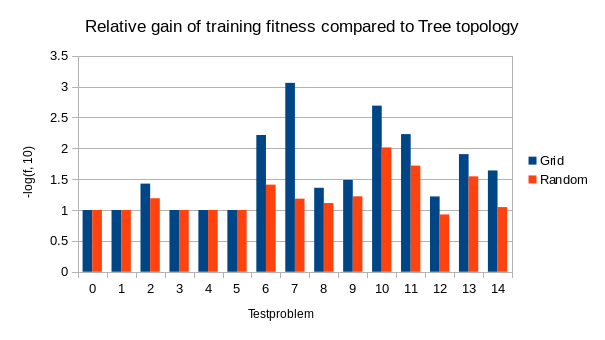
\includegraphics[width=0.8\linewidth]{figures/distributedbesttraining.png}
        \caption{Relative gain in best fitness of training data}
    \end{subfigure}%
    \begin{subfigure}{0.6\textwidth}
    \centering
        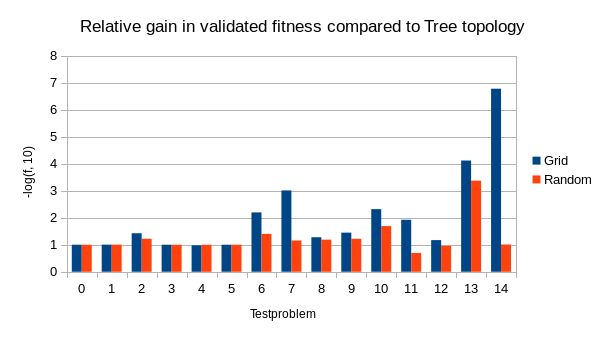
\includegraphics[width=0.8\linewidth]{figures/distributedbestvalidated.png}
        \caption{Relative gain in best fitness on full data.}
    \end{subfigure}
        \begin{subfigure}{0.6\textwidth}
    \centering
        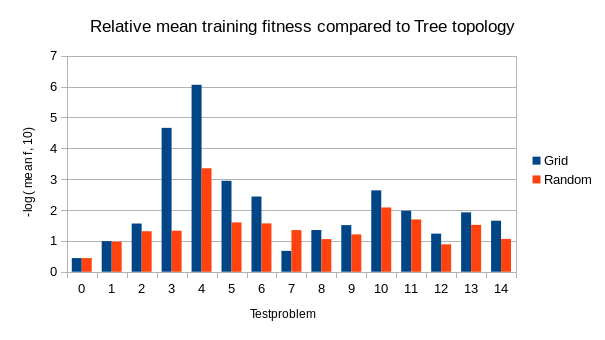
\includegraphics[width=0.8\linewidth]{figures/distributedmeantraining.png}
        \caption{Relative gain in mean fitness on training data.}
    \end{subfigure}%
    \begin{subfigure}{0.6\textwidth}
    \centering
        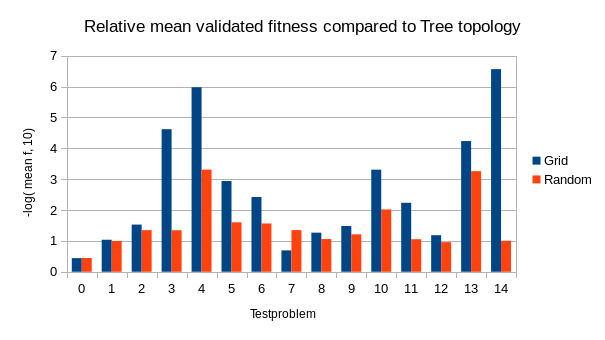
\includegraphics[width=0.8\linewidth]{figures/distributedmeanvalidated.png}
        \caption{Relative gain in mean fitness on full data.}
    \end{subfigure}
    \caption{Convergence differences between topologies.}
    \label{fig:distributedresults}
    \end{figure}
In Figure \ref{fig:distributedresults} we see how the topology affects convergence. The first observation we make is that the first 5 testproblems, with exception of the second, all have identical values for best fitness on training and validation data. The processes converged to zero fitness values for these problems, hence the identical results. 
The training fitness results in Figure \ref{fig:distributedresults}a indicate that the grid and random topology have superior convergence characteristics compared to the tree topology, with grid outperforming random on several testproblems. When we look at the fitness values on the validation data in Figure \ref{fig:distributedresults}b we see a more nuanced result. The grid topology is overall still the best choice, but the random topology has worse results for problems 11 and 12.
Next we look at the mean fitness values on training and validation data. Interestingly enough for problem 0 both random and grid score far worse than the tree topology. Overall the grid topology is still better for most problems, with the exception of problem 7. Note the similarity in pattern in the results here between training and validation data indicating that the predictive capability of the results is still good. If overfitting would have taken place we would see a reverse pattern in the results for the validation data.

\paragraph{Overhead}
Given that the Tree, Random and Grid topologies have different synchronization and memory constraints we now look at their real life overhead and discuss the results.

\subparagraph{Synchronization}
From our discussion in \ref{subasync} we know that cycles in the topology will lead to excessive synchronization and even serialization.
We measure the mean execution time for testproblem 6. The convergence characteristics using the three topologies differed significantly making this a good testcase. The processes will communicate 25 times. If the runtime of a single phase is too long, the overhead of communication will become hard to measure. If it is too short the overhead dominates the entire runtime. This second case is one we should try to avoid, it will unfairly penalize topologies with cycles forcing them to serialize. The runtime of a phase is dependent on the generations, population and depth ranges of the expressions. Ideally we would like for a practitioner to choose these parameters based on the problem at hand and not be constrained by synchronization considerations.
We compare the three topologies and use the disconnected or 'none' topology as a reference point, which has zero synchronization overhead.
This last topology has an ideal speedup of n, where n is the processcount, compared to a sequential process. From the synchronization overhead we can then derive the speedup each of the topologies is able to offer. In practice even the 'none' topology will have some synchronization overhead, as the root process has to collect all results from the other processes.
\begin{figure}
    \centering
    \begin{subfigure}{0.6\textwidth}
    \centering
        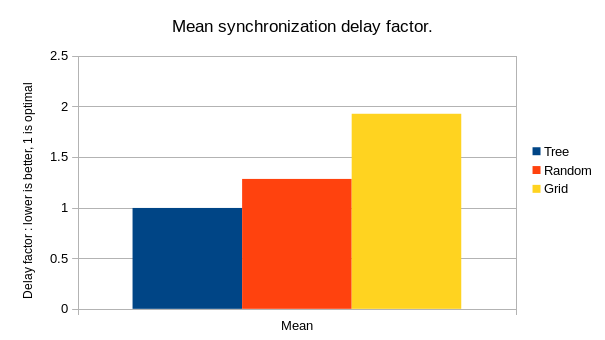
\includegraphics[width=0.8\linewidth]{figures/distributeddelaymean.png}
        \caption{Mean synchronization delay factor.}
    \end{subfigure}%
    \begin{subfigure}{0.6\textwidth}
    \centering
        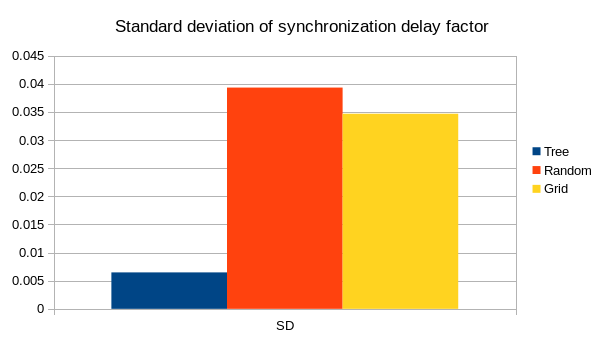
\includegraphics[width=0.8\linewidth]{figures/distributeddelaysd.png}
        \caption{Standard deviation of synchronization delay factor.}
    \end{subfigure}
    \caption{Synchronization overhead introduced by topologies.}
    \label{fig:distributeddelayresults}
    \end{figure}
In Figure \ref{fig:distributeddelayresults} we see that the tree topology has a near zero delay introduced by the synchronization. This is due to the delay tolerance we have built in in our implementation as seen in Figure \ref{fig:delaynoncyclic}. The random topology has a mean delay factor of 1.3, the grid topology scores worst with a mean delay factor of nearly 2. This is easily translated in terms of speedup. A tree topology will have near linear speedup, a grid will have a speedup roughly half of that value and a random topology will have a speedup bracketed between those two. The standard deviation for the tree topology is significantly smaller indicating that a tree topology will have a far more predictable speedup.

\subparagraph{Memory}
Memory overhead is hard to measure in a language with a garbage collector. We can estimate the overhead by calculating the needed memory in function of depth and topology used.
Let the depth be constrained by [$d_i, d_x$], with n processes, m communicationsize and a distribution spreading policy. $D_i$ is the minimum depth and $d_x$ the maximum depth. If we let $d_a = \frac{d_i + d_x}{2}$ be the average depth, then the memory requirements on average for each topology are then given by
\begin{itemize}
\item Tree : $d_a \frac{m}{2} (n-1)$
\item Random : $d_a \frac{m} n$
\item Grid : $d_a \frac{m}{4} 4 n$
\end{itemize}
Note that $d_i$ is not necessarily equal to the initial depth. While rare, it is possible that CSRM evolves trees with a depth lower than the initial depth. Unless we constrain the operators from doing so trees will start with a depth of $d_i$ but then vary between 1 and $d_x$.
Here m $>=$ 4 for a grid if we use distributing spreading policy. This leads us to an important observation. The Tree topology can communicate expressions with an average depth that is 2 times greater than the one used by the grid with the same memory usage. This factor is important, an increase in depth has an exponential effect on the complexity of the entire algorithm but also allows for more complex solutions. In addition an increased depth tolerates more bloat without losing accuracy. 
\subsection{Conclusion}
\subsubsection{Operator cooling schedule}
We have demonstrated that a cooling schedule for the mutation operator can predict and avoid mutations that are unlikely to improve fitness. This approach has a small effect on convergence but can save computationally expensive operator applications.
\subsubsection{Constant folding}
Folding constant subtrees leads to savings in the tree representation and prevents forming of ever increasingly large constant subtrees. The effects on convergence are ambiguous, the folding approach can both lead to increase as well as decrease in fitness. This depends highly on the problem and the stage at which folding is applied. 
\subsubsection{Optimizers}
The experiments with the optimizers highlight several issues. There are a wide number of strategies and parameters that influence the effect of the optimizer. We also see that optimizers can hinder the algorithm in its convergence. This is not a general conclusion, but dependent in part on our design choices and the trade-offs made. If we only optimize the final outcome of the algorithm it is obvious that no fitness regression is possible. Only when we apply optimization in the archiving stage are there subtle effects at play that allow for such edge cases. The cost of applying the optimizers is significant. In our implementation the cost is known beforehand, but the gain is not. This holds true in general for this GP SR algorithm. While we can empirically investigate the convergence of a number of problems, there is no known limit to this process. 
In general, when the optimizers are used the improvements made are far greater than the loss in edge cases. We have tested 3 distinct algorithms as optimizers in order to test which is best. Unfortunately no such algorithm exists. The NFL theorem \cite{NFL} suggests as much. What we can see is that ABC and DE offer, for our problem set, the best results. Best in this context means the overall highest gain with the lowest losses at an equal cost to the other algorithms. The hardness of the SR problem indicates that, unfortunately, there are an infinite number of problem statements that will have different convergence characteristics. While hybridization of the GP algorithm with other algorithms is a viable strategy, it also substantially increases the number of parameters. 
\subsubsection{Distributed}
We have seen that a tree topology is able to offer a near linear speedup at the cost of a lower convergence rate. As the depth increases, the synchronization between processes decreases allowing for a better speedup. The distance in phases between processes will be at most the depth of the tree.
The random and grid topologies on the other hand can offer better convergence rates but require a longer runtime in order to achieve those values. A tree topology is able to communicate expressions with average depth twice that of the grid topology making it an attractive choice for practitioners. The random topology finds a balance between the characteristics of the tree and grid, but is non deterministic in its communication patterns. The resulting convergence and runtime will be influenced by each new random communication pattern, leading to uncertainty for the practitioner.
 
\section{Use Case}
In this section we will use our tool on a real world use case. % ref stride
% Ref stride, quickly what it is, why our tool, what's the results ?
\subsection{Problem statement}
We want to use symbolic regression on the output of a simulator. The parameter space of the simulator is huge, and a single simulation instance is computationally expensive. We would like to obtain symbolic expressions relating parameters values to simulator output. These expressions can be used to gain insight into which parameters are correlated, which have a larger effect on output and which are irrelevant. 
Given the huge parameter space of the simulator a Design Of Experiment is constructed where the coverage of the parameter space is maximized while minimizing the number of combinations for all parameters. % rewrite this when I have some caffeine in my blood
We then execute the simulator on each configuration. With the execution of a single configuraton independent of all others this is an embarrassingly parallel problem. We combine the output of all configurations and feed them into a tool where we can apply symbolic regression or another machine learning technique in order to extract a model that approximates the simulator. The problem with this approach is twofold. We have to wait until the simulator has completed all configurations and the SR tool executes on a large dataset. It has no known starting point so effectively performs a blind search in a huge search space. We can avoid both issues by using partial results from the simulator as input for the SR tool. The results from these partial samples ideally will provide a good starting point for the incrementally growing dataset. The last assumption only holds if the sequence of completed configurations is a good sample of the full dataset. We can enforce this sequence by ordering the configurations but this is non trivial. Configurations will not have the same computational load for all simulations. Consider for example the population parameter in a epidemiological simulator. An increase in runtime is expected if we increase this parameter. Even if we take this into account in our scheduling, the parallel execution of any number of tasks is never deterministic. The order of configurations is not only important to avoid a bias for the full design, which would lead to overfitting. The initialization problem \ref{subsubinvalidexpressions} reappears here. If the initial partial set of configurations is biased the probability is quite high that the resulting solutions are invalid for the complete data set. 
\subsection{Design of Experiment}
% List DOE technique used and parameter configuration
% Why this technique
\subsubsection{Experiment configuration}
We construct a DOE with 3 parameters, 30 points in total. 
\begin{itemize}
\item initial depth 3
\item maximum depth 6
\item p: population 20
\item g: generations per phase 60
\item f: phases 30
\item archive 4 best per phase
\item d: datapoints : 10, 20, 30
\end{itemize}
The total cost in fitness evaluations is then given by: 20*60*30*d.
We compare 3 approaches. First we run the CSRM tool on the entire dataset. This is the classical approach, the tool is not seeded and so starts a blind search. In a real world setting this would mean waiting until the simulator has run all 30 configurations.
In our second approach we split the data into incremental sections. After 10 configurations have completed we start the tool on this dataset. 
The best 4 results are saved to disk, then we run the tool with the result of 20 configurations and use the results from the previous run as a seed. The overlap between the two datasets will mitigate the initialization problem. Finally we use the results of the 20-point dataset as seed for the 30 point run. 
The cost of running the 10 and 20 point runs to use as seed for the 30 point run is equal to the cost of the 30 point run. 
To ground the comparision our last approach runs the tool on the data from 30 configurations with double the amount of phases. This means that it has the same number of fitness evaluations as the 10-20-30 combination. We compare all three to see which gains are made and at what cost.
\subsection{Results}
\subsubsection{Fitness improvement}
In Figure \ref{fig:incrementalgain} we see that the fitness is improved by using the best results of the previous run on a partial data set. We have deliberately split our data set to expose a risk here. If we run the tool with 20 datapoints seeded by a run of 10 datapoints, we see that the validated fitness actually decreases compared to a non seeded run. The ratio between new and known data is too large, leading to overfitting. If we seed the best results from the 20-point run into a 30 point configuration we see that both the training and validated fitness values significantly improve. 
The 30 point run with 60 phases has the same computational cost as the 10-20-30 runs combined, but has lower convergence. We see that convergence is slowing, with training fitness improving by a factor of 1.1, but validation fitness worsens. This is a typical example of overfitting. The combined 10-20-30 run increases validation fitness with a factor of 1.13. Note the clustering patterns in the incremental runs. When seeded with solutions of previous runs we introduce information that the algorithm otherwise would have to discover. These seeds have fitness values somewhere between the randomly generated and optimal samples. Applying operators on them leads to a niching effect visualized in the fitness distribution. Seeding will not guarantee this effect, it is a possibility depending on how the seeds fit in the trajectory in the search space that the algorithm generate during its execution.
\begin{figure}
    \centering
    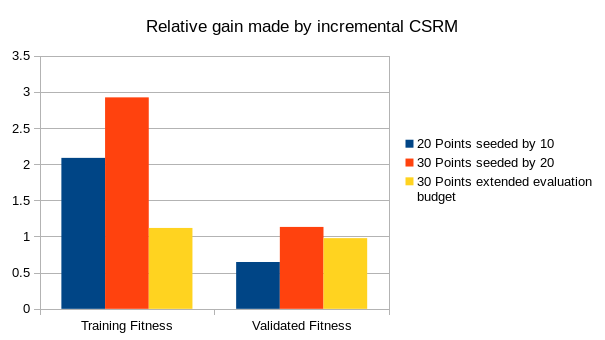
\includegraphics[width=\textwidth,height=\textheight,keepaspectratio]{figures/incrementalgain.png}
    \caption{Incremental fitness gain in CSRM.}
    \label{fig:incrementalgain}
\end{figure}
\subsubsection{Convergence behavior}
\paragraph{Fitness distribution}
In Figures \ref{fig:incrementalseededconvergence}\ref{fig:incrementalconvergence}\ref{fig:incrementaldoubleconvergence} we see how the convergence process evolves over time. If we compare the fitness plot we clearly see that the seeded process has a different distribution compared with the unseeded runs. Around generation 1000 the convergence rate slows. Doubling the phases has little effect on the fitness distribution. 
% TODO check plots of fitness, make sure they correspond to those runs
\paragraph{Operator effectiveness}
In the plots we see operator success rate and operator gains visualized. The first is the ratio between applications of an operator that leads to improvement in fitness versus the total number of applications. The trendline is obtained by a cubic fit.This gives us an indication whether an operator is still effective, in particular it gives us the fraction of the population that is improved each generation by the operator. The second plot is the mean gain of an operator, it reflects how much the fitness of each generation is improved by an operator. The distinction is important, if fitness is improved by very small amounts the success rate will be high but the gain low. These statistics offer an insight into the convergence characteristics over generations. Instead of relying only on the end result we can directly observe the effects of the operators. For our comparison we see that there is little difference in gain or success rate between the three runs.
\paragraph{Constant folding}
The percentage of nodes saved is similar for all three runs. The plots show that constant subtrees are introduced at a constant rate and folded at the end of each generation. The savings plotted also give an indication of the potential increase in nodes that could take place if folding was not implemented. 
 \begin{figure}
    \begin{subfigure}{0.5\textwidth}
        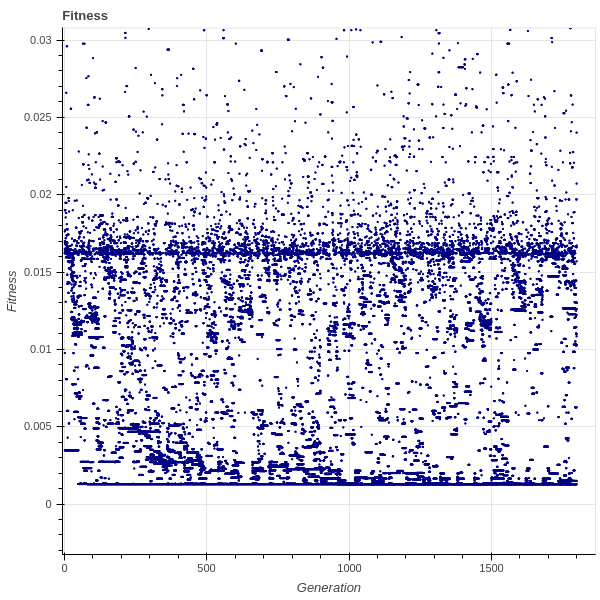
\includegraphics[width=0.8\linewidth]{figures/incrementalfitness30s.png}
        \caption{Fitness.}
    \end{subfigure}
    \begin{subfigure}{0.5\textwidth}
        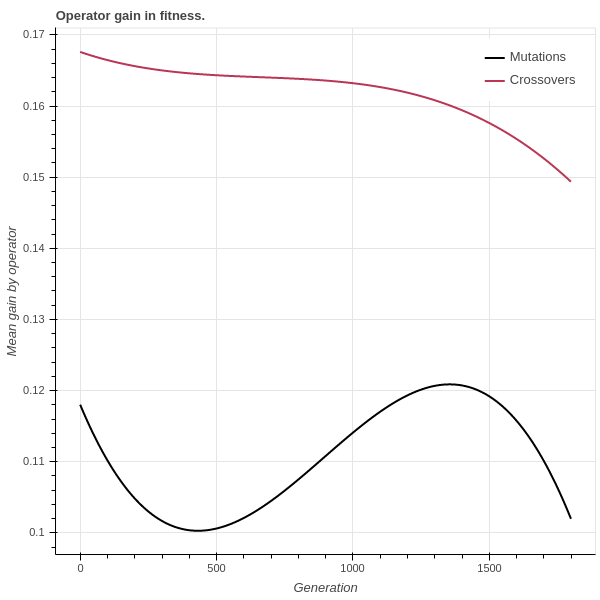
\includegraphics[width=0.8\linewidth]{figures/incrementaloperatorgain30s.png}
        \caption{Operator gain.}
    \end{subfigure}
        \begin{subfigure}{0.5\textwidth}
        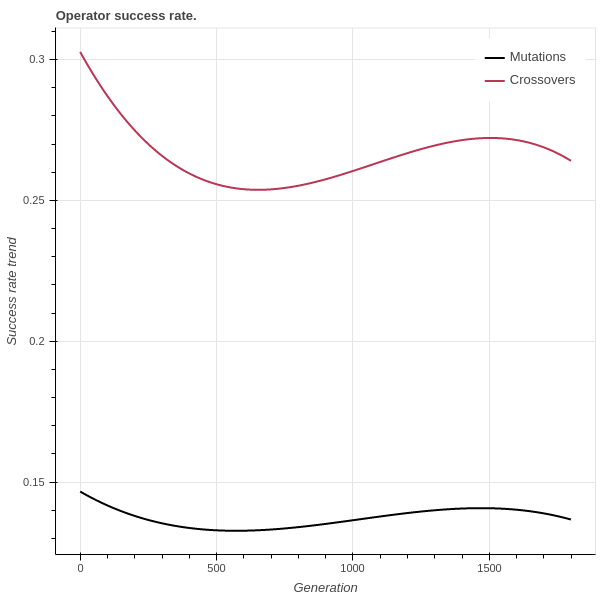
\includegraphics[width=0.8\linewidth]{figures/incrementaloperatorsuccessrate30s.png}
        \caption{Operator success rate.}
    \end{subfigure}
    \begin{subfigure}{0.5\textwidth}
        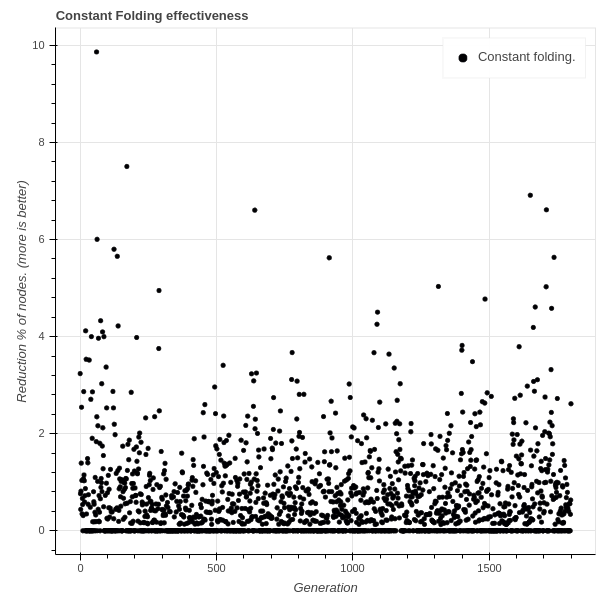
\includegraphics[width=0.8\linewidth]{figures/incrementalconstfolding30s.png}
        \caption{Constant folding savings.}
    \end{subfigure}
    \caption{Convergence behavior of incremental symbolic regression with 10-20-30 split.}
    \label{fig:incrementalseededconvergence}
\end{figure}
 \begin{figure}
    \begin{subfigure}{0.5\textwidth}
        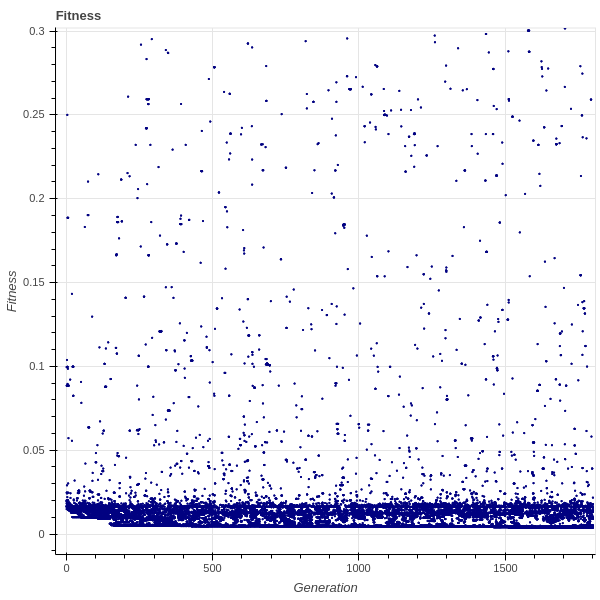
\includegraphics[width=0.8\linewidth]{figures/incrementalfitness30.png}
        \caption{Fitness.}
    \end{subfigure}
    \begin{subfigure}{0.5\textwidth}
        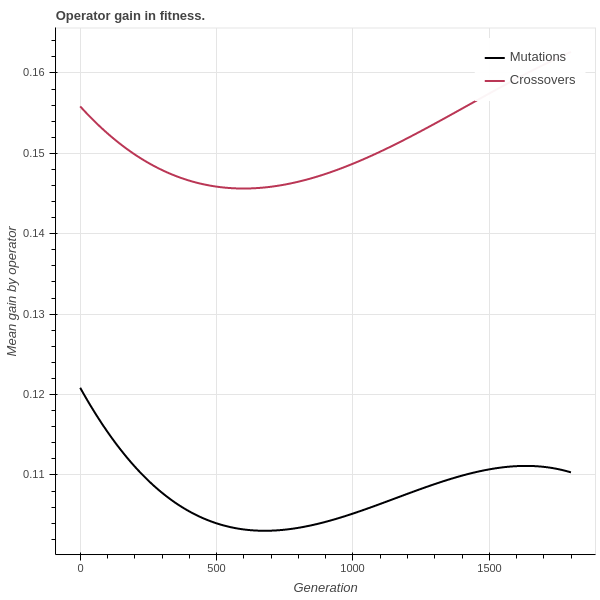
\includegraphics[width=0.8\linewidth]{figures/incrementaloperatorgain30.png}
        \caption{Operator gain.}
    \end{subfigure}
        \begin{subfigure}{0.5\textwidth}
        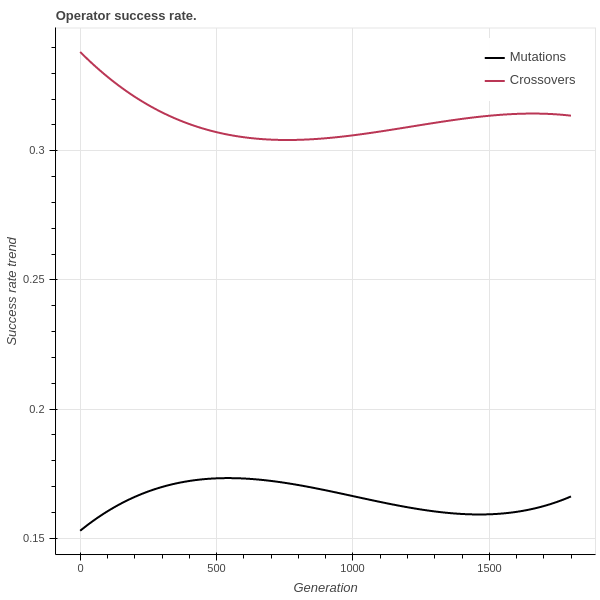
\includegraphics[width=0.8\linewidth]{figures/incrementaloperatorsuccessrate30.png}
        \caption{Operator success rate.}
    \end{subfigure}
    \begin{subfigure}{0.5\textwidth}
        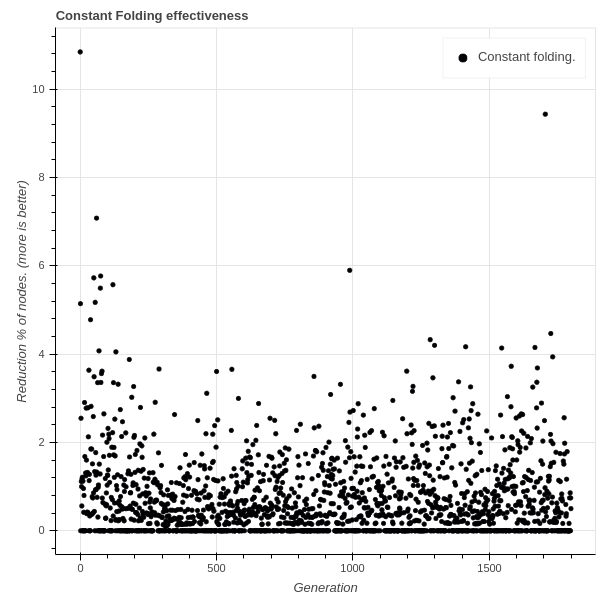
\includegraphics[width=0.8\linewidth]{figures/incrementalconstfolding30.png}
        \caption{Constant folding savings.}
    \end{subfigure}
    \caption{Convergence behavior of incremental symbolic regression without split.}
    \label{fig:incrementalconvergence}
\end{figure}
% [bcardoen@localhost src]$ python3 -m gp.paralleldriver -c 1 -t none -g 60 -p 20 -f 60 -x doe/input.csv -y doe/output.csv -m 6 -v -d 30 -q 3 -i 3

 \begin{figure}
    \begin{subfigure}{0.5\textwidth}
        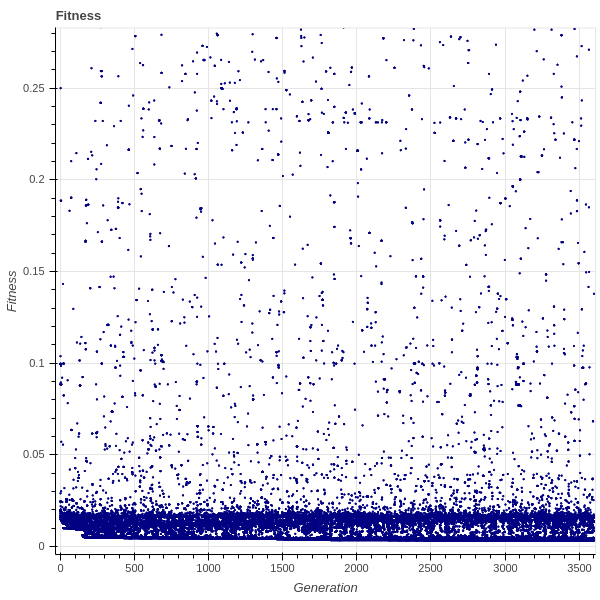
\includegraphics[width=0.8\linewidth]{figures/incrementalfitness30d.png}
        \caption{Fitness.}
    \end{subfigure}
    \begin{subfigure}{0.5\textwidth}
        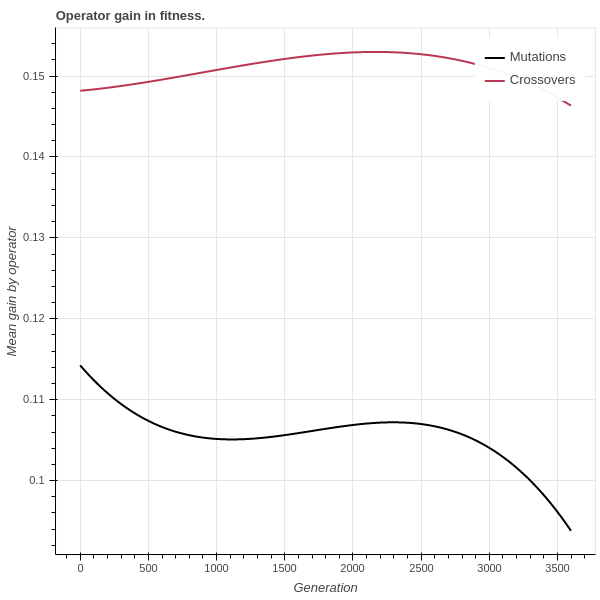
\includegraphics[width=0.8\linewidth]{figures/incrementaloperatorgain30d.png}
        \caption{Operator gain.}
    \end{subfigure}
        \begin{subfigure}{0.5\textwidth}
        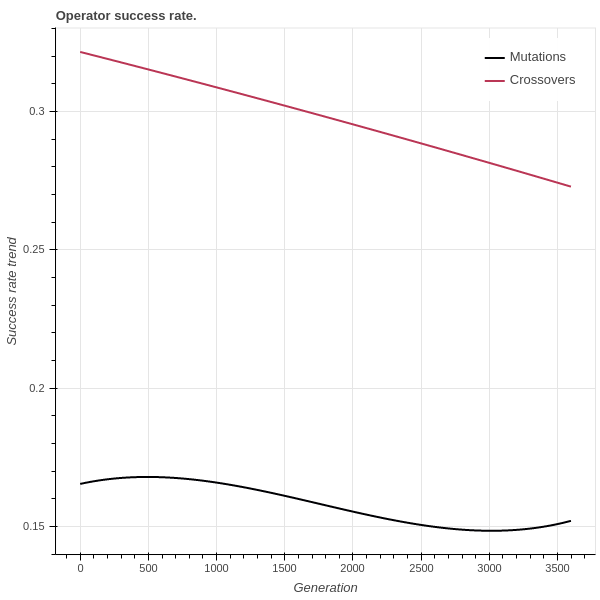
\includegraphics[width=0.8\linewidth]{figures/incrementaloperatorsuccessrate30d.png}
        \caption{Operator success rate.}
    \end{subfigure}
    \begin{subfigure}{0.5\textwidth}
        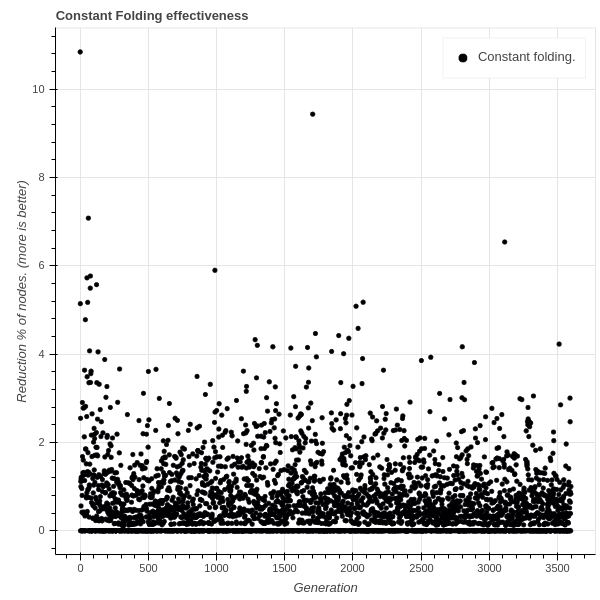
\includegraphics[width=0.8\linewidth]{figures/incrementalconstfolding30d.png}
        \caption{Constant folding savings.}
    \end{subfigure}
    \caption{Convergence behavior of incremental symbolic regression with identical computational cost as 10-20-30 split.}
    \label{fig:incrementaldoubleconvergence}
\end{figure}
\subsection{Conclusion}
We have seen that incremental use of symbolic regression can, when applied judiciously, increase convergence compared to a blind search with the same computational cost. In addition to obtaining improved results we can integrate it with a simulator that produces output in parallel.


\section{Conclusion}
We have introduced a distributed SR tool with a delay tolerance mechanism that mitigates load imbalance between processes. We have compared three representative topologies in terms of convergence rate and speed-up. The tree topology can be used as an approximation for the grid topology with near linear speed-up and offers a process a delay tolerance equal to the distance between dependent processes. This feature improves the tree topology to scale when the process set is larger. The distributed processes approximate K fold cross validation (KCV) in order to avoid overfitted solutions without its computational cost. Our modular architecture allows the tool to be extended with new topologies, policies, and optimization algorithms. 

In a use case we have demonstrated the use our tool can be used to build a surrogate models for a simulator in an incremental approach, i.e. concurrent to the simulator running over all input data sets. For the use case, it lead to improvements in fitness and predictive value of the final model. A feedback loop between practitioner, simulator and regression tool offers savings in time while yielding insights that can be used by domain experts to enhance the model building. The use case demonstrated that intermediate solutions are able to approximate the final model's characteristics sufficiently to be of value, thus validating our incremental approach. 

The distributed results of the use case were in line with the results of the benchmarks. The grid topology obtained the highest quality solution at the lowest speed-up. The tree topology achieved a near linear speed-up at the cost of a lower quality solution. The random topology demonstrated that the incremental approach can lead to overfitting in a distributed setting. 

Future work can take any of three directions. First our distributed architecture allows for a each process to use a different metaheuristic, creating a heterogeneous set of communicating algorithms. A cooperative set of optimizations algorithms could offer an optimal solution for all problem instances by balancing the disadvantages and advantages of each algorithm. 
Second, the tool can easily be extended with new topologies and spreading policies to further investigate their effects on convergence and accuracy. Lastly, we can approximate incremental design of experiment by making use of the collapsing property of latin hypercubes. By reducing the number of parameters and fixing the other values, we could avoid the naive linear division approach we thus far have used in seeding the tool and possibly maintain the space filling characteristics of the LHD.


% no \IEEEPARstart
%This demo file is intended to serve as a ``starter file''
%for IEEE conference papers produced under \LaTeX\ using
%IEEEtran.cls version 1.8b and later.
%% You must have at least 2 lines in the paragraph with the drop letter
%% (should never be an issue)
%I wish you the best of success.
%
%\hfill mds
% 
%\hfill August 26, 2015
%
%\subsection{Subsection Heading Here}
%Subsection text here.
%
%
%\subsubsection{Subsubsection Heading Here}
%Subsubsection text here.


% An example of a floating figure using the graphicx package.
% Note that \label must occur AFTER (or within) \caption.
% For figures, \caption should occur after the \includegraphics.
% Note that IEEEtran v1.7 and later has special internal code that
% is designed to preserve the operation of \label within \caption
% even when the captionsoff option is in effect. However, because
% of issues like this, it may be the safest practice to put all your
% \label just after \caption rather than within \caption{}.
%
% Reminder: the "draftcls" or "draftclsnofoot", not "draft", class
% option should be used if it is desired that the figures are to be
% displayed while in draft mode.
%
%\begin{figure}[!t]
%\centering
%\includegraphics[width=2.5in]{myfigure}
% where an .eps filename suffix will be assumed under latex, 
% and a .pdf suffix will be assumed for pdflatex; or what has been declared
% via \DeclareGraphicsExtensions.
%\caption{Simulation results for the network.}
%\label{fig_sim}
%\end{figure}

% Note that the IEEE typically puts floats only at the top, even when this
% results in a large percentage of a column being occupied by floats.


% An example of a double column floating figure using two subfigures.
% (The subfig.sty package must be loaded for this to work.)
% The subfigure \label commands are set within each subfloat command,
% and the \label for the overall figure must come after \caption.
% \hfil is used as a separator to get equal spacing.
% Watch out that the combined width of all the subfigures on a 
% line do not exceed the text width or a line break will occur.
%
%\begin{figure*}[!t]
%\centering
%\subfloat[Case I]{\includegraphics[width=2.5in]{box}%
%\label{fig_first_case}}
%\hfil
%\subfloat[Case II]{\includegraphics[width=2.5in]{box}%
%\label{fig_second_case}}
%\caption{Simulation results for the network.}
%\label{fig_sim}
%\end{figure*}
%
% Note that often IEEE papers with subfigures do not employ subfigure
% captions (using the optional argument to \subfloat[]), but instead will
% reference/describe all of them (a), (b), etc., within the main caption.
% Be aware that for subfig.sty to generate the (a), (b), etc., subfigure
% labels, the optional argument to \subfloat must be present. If a
% subcaption is not desired, just leave its contents blank,
% e.g., \subfloat[].


% An example of a floating table. Note that, for IEEE style tables, the
% \caption command should come BEFORE the table and, given that table
% captions serve much like titles, are usually capitalized except for words
% such as a, an, and, as, at, but, by, for, in, nor, of, on, or, the, to
% and up, which are usually not capitalized unless they are the first or
% last word of the caption. Table text will default to \footnotesize as
% the IEEE normally uses this smaller font for tables.
% The \label must come after \caption as always.
%
%\begin{table}[!t]
%% increase table row spacing, adjust to taste
%\renewcommand{\arraystretch}{1.3}
% if using array.sty, it might be a good idea to tweak the value of
% \extrarowheight as needed to properly center the text within the cells
%\caption{An Example of a Table}
%\label{table_example}
%\centering
%% Some packages, such as MDW tools, offer better commands for making tables
%% than the plain LaTeX2e tabular which is used here.
%\begin{tabular}{|c||c|}
%\hline
%One & Two\\
%\hline
%Three & Four\\
%\hline
%\end{tabular}
%\end{table}


% Note that the IEEE does not put floats in the very first column
% - or typically anywhere on the first page for that matter. Also,
% in-text middle ("here") positioning is typically not used, but it
% is allowed and encouraged for Computer Society conferences (but
% not Computer Society journals). Most IEEE journals/conferences use
% top floats exclusively. 
% Note that, LaTeX2e, unlike IEEE journals/conferences, places
% footnotes above bottom floats. This can be corrected via the
% \fnbelowfloat command of the stfloats package.


% trigger a \newpage just before the given reference
% number - used to balance the columns on the last page
% adjust value as needed - may need to be readjusted if
% the document is modified later
%\IEEEtriggeratref{8}
% The "triggered" command can be changed if desired:
%\IEEEtriggercmd{\enlargethispage{-5in}}

% references section

% can use a bibliography generated by BibTeX as a .bbl file
% BibTeX documentation can be easily obtained at:
% http://mirror.ctan.org/biblio/bibtex/contrib/doc/
% The IEEEtran BibTeX style support page is at:
% http://www.michaelshell.org/tex/ieeetran/bibtex/
%\bibliographystyle{IEEEtran}
% argument is your BibTeX string definitions and bibliography database(s)
%\bibliography{IEEEabrv,../bib/paper}
%
% <OR> manually copy in the resultant .bbl file
% set second argument of \begin to the number of references
% (used to reserve space for the reference number labels box)
%\begin{thebibliography}{1}
%
%\bibitem{IEEEhowto:kopka}
%H.~Kopka and P.~W. Daly, \emph{A Guide to \LaTeX}, 3rd~ed.\hskip 1em plus
%  0.5em minus 0.4em\relax Harlow, England: Addison-Wesley, 1999.
%
%\end{thebibliography}

\bibliographystyle{IEEEtran}
\bibliography{papers}


% that's all folks
\end{document}


